\chapter{Résultats et Discussion}
\label{chap:resultats}

% ─────────────────────────────────────────────────────────────────────────────
\section{Résultats de l'analyse exploratoire (EDA)}
% ─────────────────────────────────────────────────────────────────────────────

\subsection{Statistiques descriptives du dataset nettoyé}

Après l'étape de binarisation BRFSS et de déduplication, le dataset présente
les statistiques descriptives du tableau~\ref{tab:stats_eda}.

\begin{table}[H]
\centering
\caption{Statistiques descriptives du dataset nettoyé (n = 1\,760\,241)}
\label{tab:stats_eda}
\begin{tabular}{lrrrrr}
\toprule
\textbf{Variable} & \textbf{Moyenne} & \textbf{Médiane} & \textbf{Écart-type} & \textbf{Min} & \textbf{Max} \\
\midrule
BMI            & 28,38 &  27,54 &  6,25 & 12,0 & 98,0 \\
GenHlth        &  2,52 &   2,00 &  1,09 &  1,0 &  5,0 \\
Age            &  8,42 &   9,00 &  2,87 &  1,0 & 13,0 \\
MentHlth       &  3,47 &   0,00 &  7,89 &  0,0 & 30,0 \\
PhysHlth       &  4,56 &   0,00 &  9,12 &  0,0 & 30,0 \\
RiskScore      &  0,82 &   1,00 &  0,91 &  0,0 &  5,0 \\
HealthIndex    &  4,02 &   3,33 &  2,21 &  1,0 & 15,0 \\
\bottomrule
\end{tabular}
\end{table}

La médiane de MentHlth et PhysHlth est égale à 0~: la majorité des répondants
déclarent aucun jour de mauvaise santé dans les 30 jours précédents, produisant
des distributions fortement asymétriques à droite. Ce comportement est cohérent
avec la littérature épidémiologique BRFSS et ne constitue pas une anomalie de données.

\subsection{Distributions univariées}

La figure~\ref{fig:univariate} présente les distributions de l'ensemble des features
numériques et ordinales, comparées entre la classe MCV (positif) et la classe
non-MCV (négatif). Cette visualisation permet d'identifier visuellement les features
les plus discriminantes avant toute modélisation.

\begin{figure}[H]
    \centering
    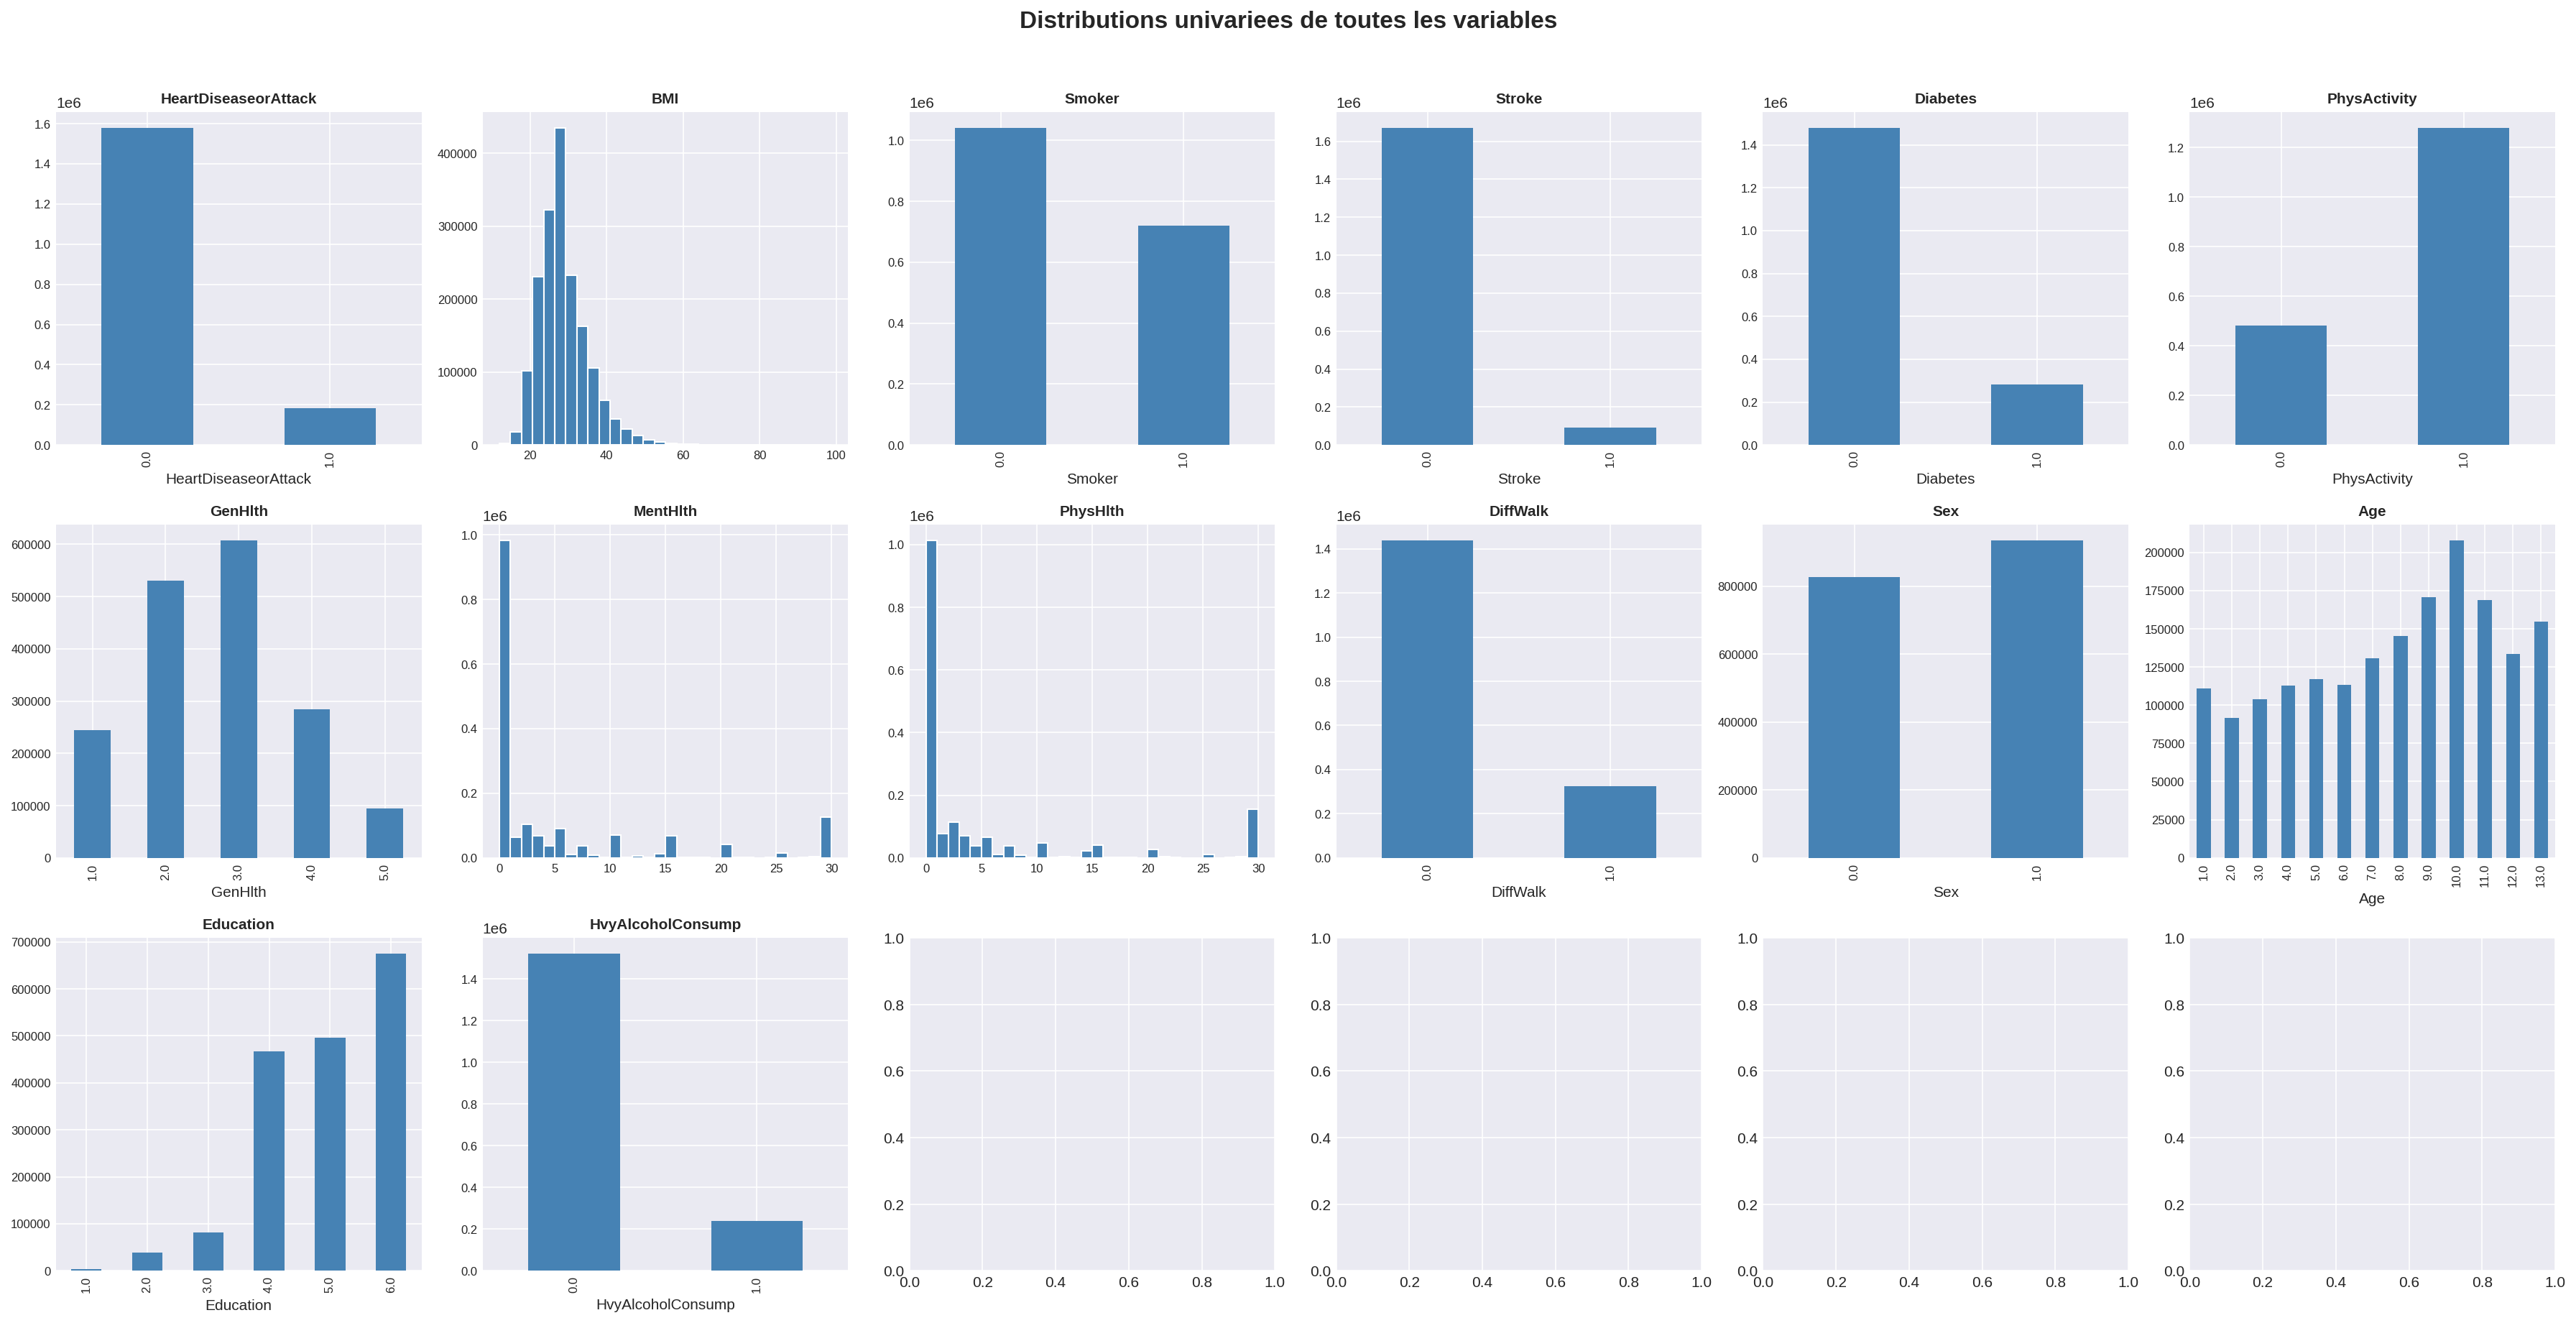
\includegraphics[width=\textwidth]{figures/univariate_distributions.png}
    \caption{Distributions univariées des features numériques et ordinales selon
             la classe cible (bleu~: non-MCV, orange~: MCV). Age, GenHlth et Stroke
             présentent les décalages les plus marqués entre classes,
             confirmant leur pouvoir discriminant.}
    \label{fig:univariate}
\end{figure}

Les observations principales sont les suivantes~:
\begin{itemize}
    \item \textbf{Age}~: les patients MCV se concentrent dans les tranches 9--13
          (55 ans et plus), avec une médiane supérieure d'environ 2 tranches
          par rapport aux non-MCV.
    \item \textbf{GenHlth}~: les patients MCV s'auto-évaluent en moins bonne santé
          (distribution décalée vers les valeurs 3--5).
    \item \textbf{BMI}~: légère différence de distribution, les MCV ayant un BMI
          médian légèrement plus élevé, mais les distributions se chevauchent
          fortement, limitant le pouvoir discriminant de cette variable seule.
\end{itemize}

\subsection{Distribution de la variable cible}

La figure~\ref{fig:target_dist} illustre le déséquilibre de classes dans le dataset
nettoyé. La classe positive (MCV diagnostiquée) représente 10,32\% des observations.

\begin{figure}[H]
    \centering
    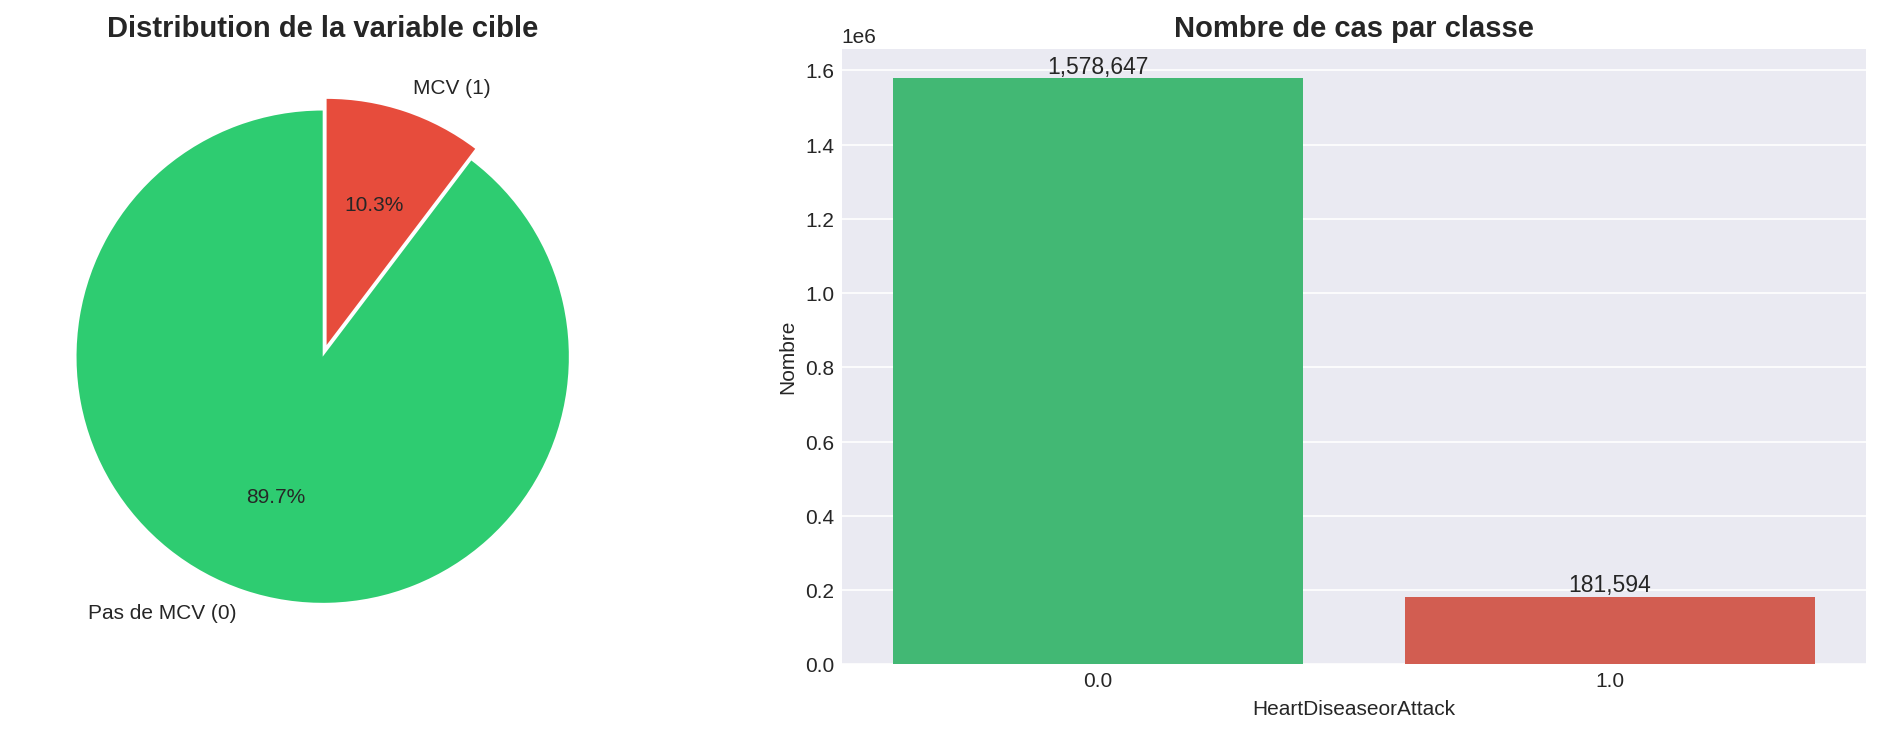
\includegraphics[width=0.75\textwidth]{figures/target_distribution.png}
    \caption{Distribution de la variable cible \texttt{HeartDiseaseorAttack}
             après nettoyage (1\,760\,241 observations). Le rapport de classes
             8,68~:~1 est inhérent à la prévalence épidémiologique réelle des MCV
             dans la population américaine adulte.}
    \label{fig:target_dist}
\end{figure}

\subsection{Analyse des corrélations}

La figure~\ref{fig:corr} présente la matrice de corrélation de Pearson sur
l'ensemble des features. Les corrélations positives les plus fortes avec la cible
sont observées pour Age (0,250), GenHlth (0,213), Stroke (0,188) et DiffWalk (0,183).
La corrélation négative la plus marquée concerne PhysActivity ($-$0,094),
confirmant l'effet protecteur de l'activité physique.

\begin{figure}[H]
    \centering
    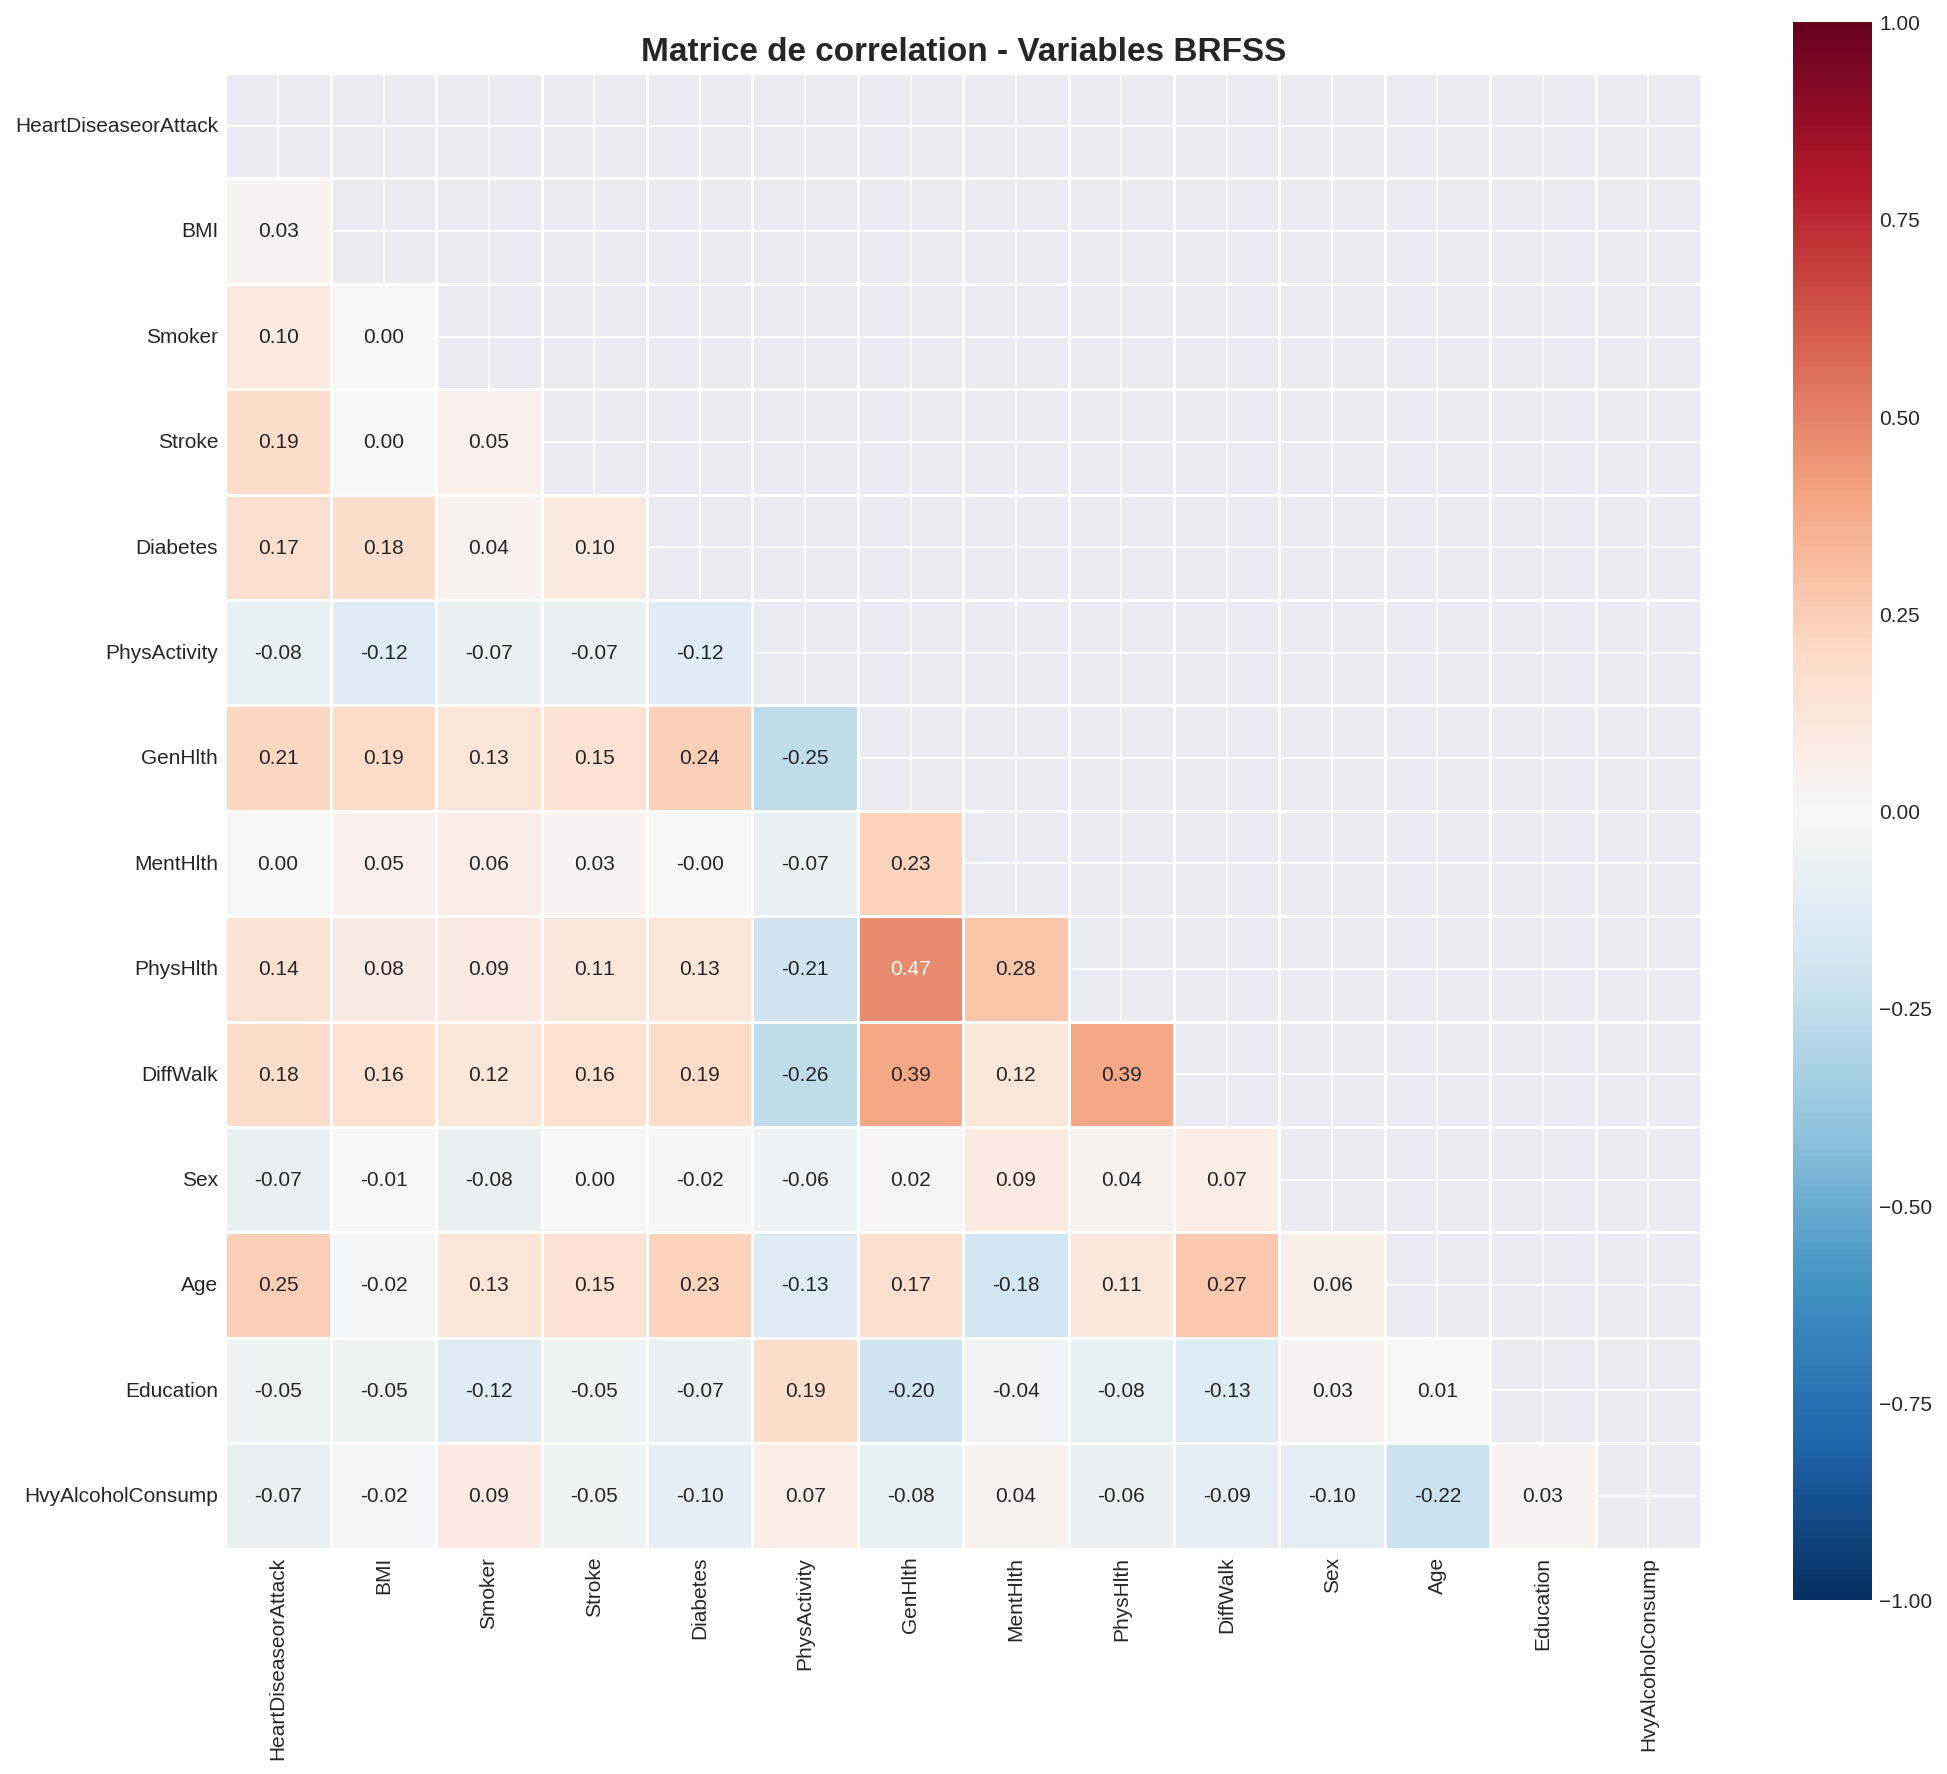
\includegraphics[width=\textwidth]{figures/correlation_heatmap.png}
    \caption{Matrice de corrélation de Pearson — dataset BRFSS 2020--2024 (n = 200\,000).
             Les corrélations entre features restent modérées (pas de multi-colinéarité
             sévère), la corrélation maximale entre prédicteurs est de 0,32
             (entre RiskScore et Stroke, attendue par construction).}
    \label{fig:corr}
\end{figure}

La figure~\ref{fig:target_correlation} compare les corrélations de chaque feature
avec la variable cible, en regard de l'importance Gini, pour mettre en évidence
les convergences et divergences entre les deux méthodes d'évaluation.

\begin{figure}[H]
    \centering
    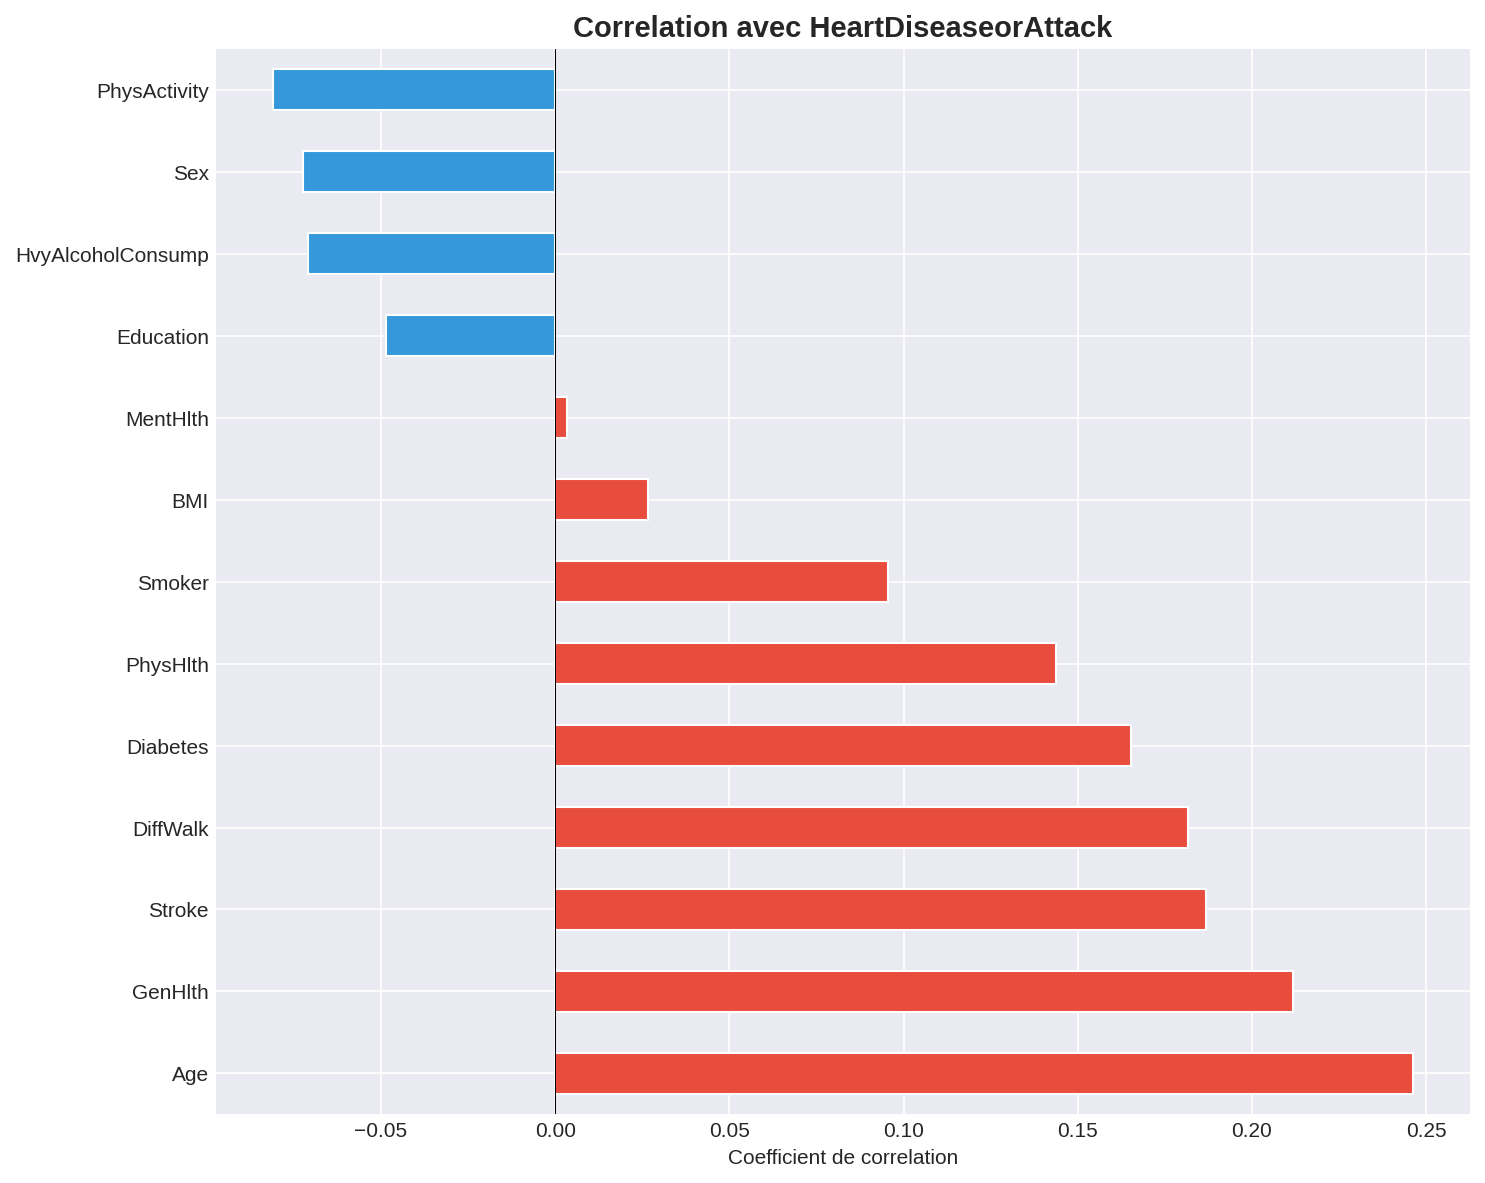
\includegraphics[width=0.85\textwidth]{figures/target_correlation.png}
    \caption{Corrélation de chaque feature avec la variable cible (axe horizontal)
             versus son importance Gini normalisée (axe vertical).
             Les features proches de la diagonale sont cohérentes entre les deux
             méthodes~; les divergences notables concernent BMI (Gini élevé,
             corrélation faible) et PhysActivity (corrélation élevée, Gini faible).}
    \label{fig:target_correlation}
\end{figure}

\subsection{Importance des features}

La figure~\ref{fig:gini} présente l'importance Gini calculée par un Random Forest
préliminaire de 100 arbres. Les trois features dominantes sont~: Age (34,06\%),
GenHlth (20,33\%) et Stroke (16,13\%), représentant à elles seules 70,5\%
de l'importance totale.

\begin{figure}[H]
    \centering
    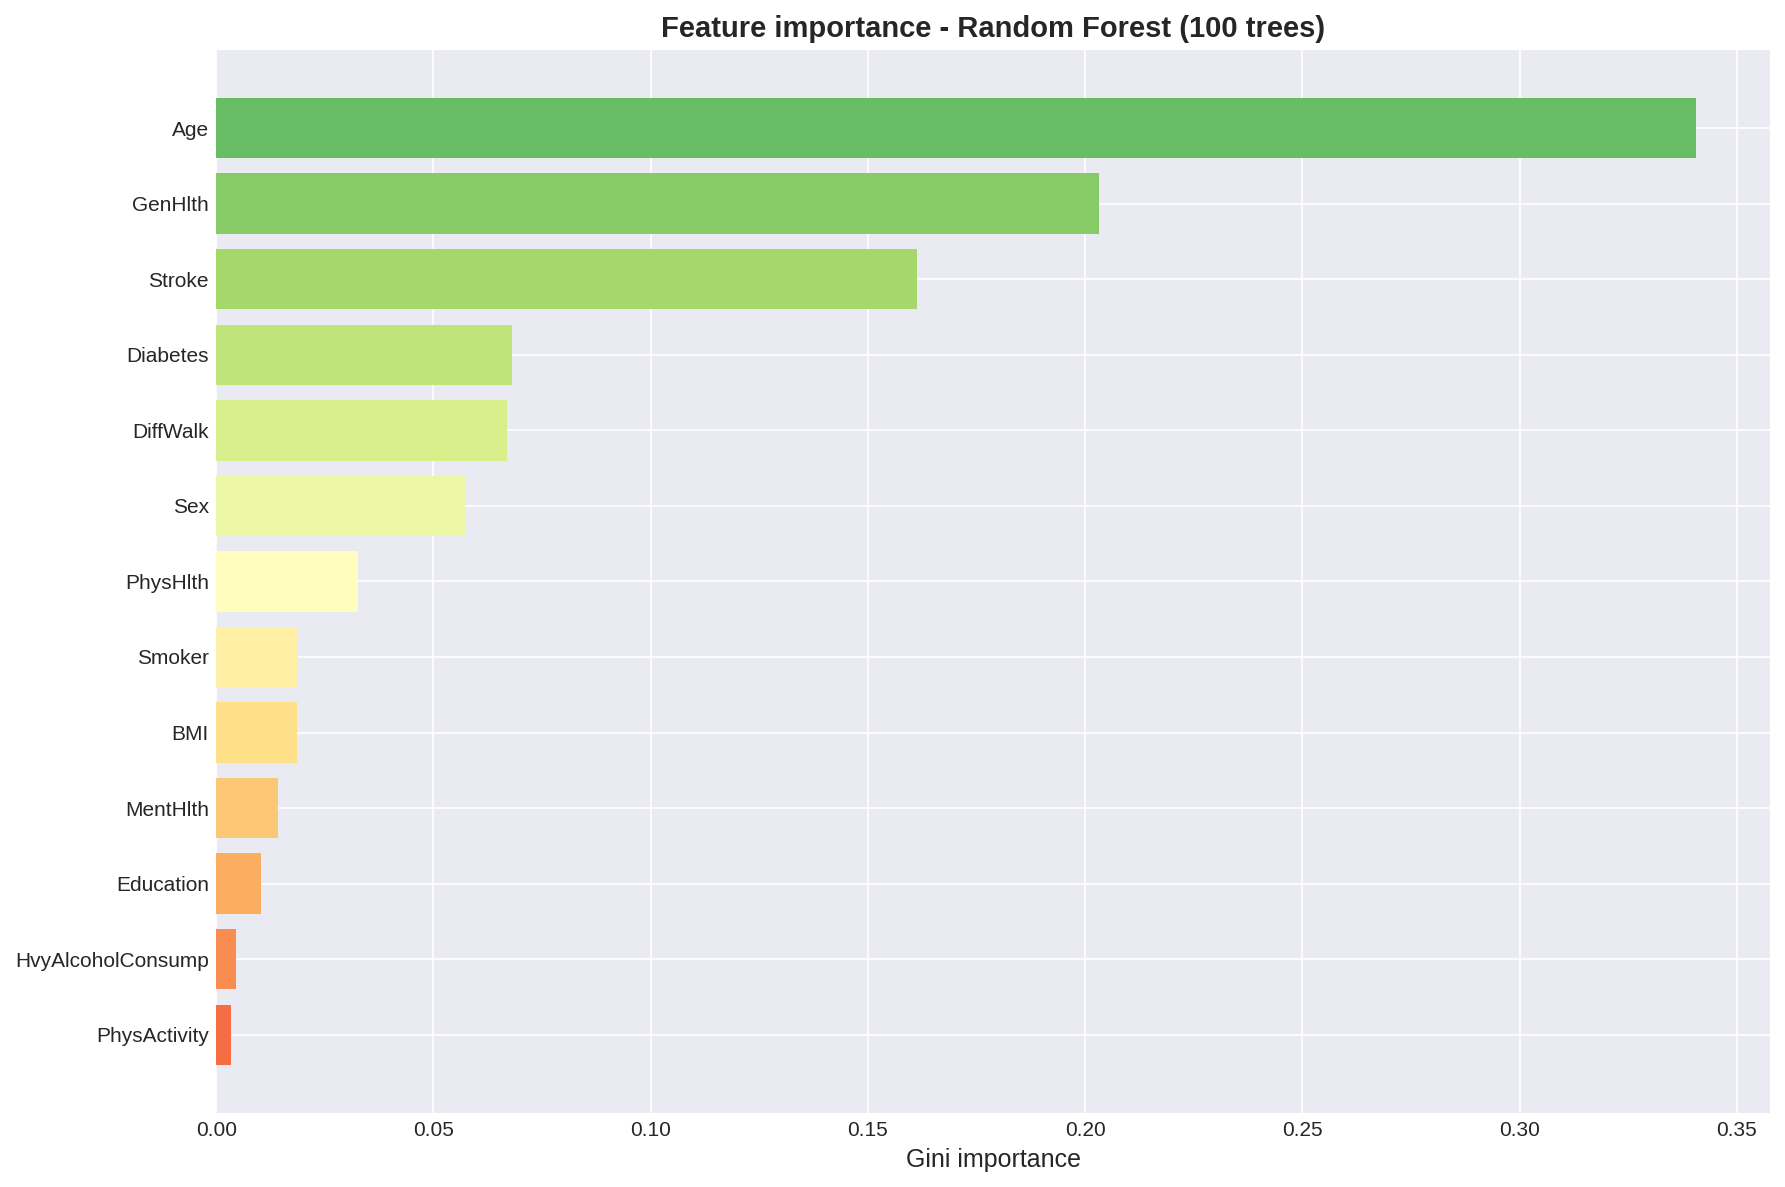
\includegraphics[width=0.85\textwidth]{figures/feature_importance_gini.png}
    \caption{Importance des features par critère de réduction d'impureté de Gini
             (Random Forest, 100 arbres, 30\% de l'échantillon). Age, GenHlth et
             Stroke dominent avec 70,5\% de l'importance totale, cohérent avec
             la littérature épidémiologique sur les facteurs de risque cardiovasculaire.}
    \label{fig:gini}
\end{figure}

% ─────────────────────────────────────────────────────────────────────────────
\section{Performances des modèles}
% ─────────────────────────────────────────────────────────────────────────────

\subsection{Comparaison globale des métriques}

\begin{table}[H]
\centering
\caption{Comparaison des performances sur le jeu de test --- DNN vs XGBoost vs Spark GBT}
\label{tab:results_comparison}
\begin{tabular}{lcccc}
\toprule
\textbf{Métrique} & \textbf{DNN ($\tau=0{,}5$)} & \textbf{DNN ($\tau=0{,}67$)} & \textbf{XGBoost} & \textbf{Spark GBT} \\
\midrule
Accuracy           & 0,698 & 0,822 & 0,701 & 0,898 \\
Précision          & 0,227 & 0,305 & 0,229 & --- \\
Rappel             & 0,802 & 0,563 & 0,799 & --- \\
F1-Score           & 0,354 & 0,396 & 0,356 & 0,860\textsuperscript{*} \\
AUC-ROC            & \multicolumn{2}{c}{0,819} & 0,820 & 0,819 \\
Temps entraîn.~(s) & \multicolumn{2}{c}{177,8} & 67,1  & 270,2 \\
Temps inférence~(s)& \multicolumn{2}{c}{0,93}  & 1,51  & 0,05 \\
\bottomrule
\multicolumn{5}{l}{\textsuperscript{*} F1 pondéré (weighted), dominé par la classe négative
                    — non comparable aux F1 binaires}
\end{tabular}
\end{table}

Les figures~\ref{fig:metrics_barchart} et~\ref{fig:metrics_radar} comparent
graphiquement les métriques des modèles sous deux représentations complémentaires.

\begin{figure}[H]
    \centering
    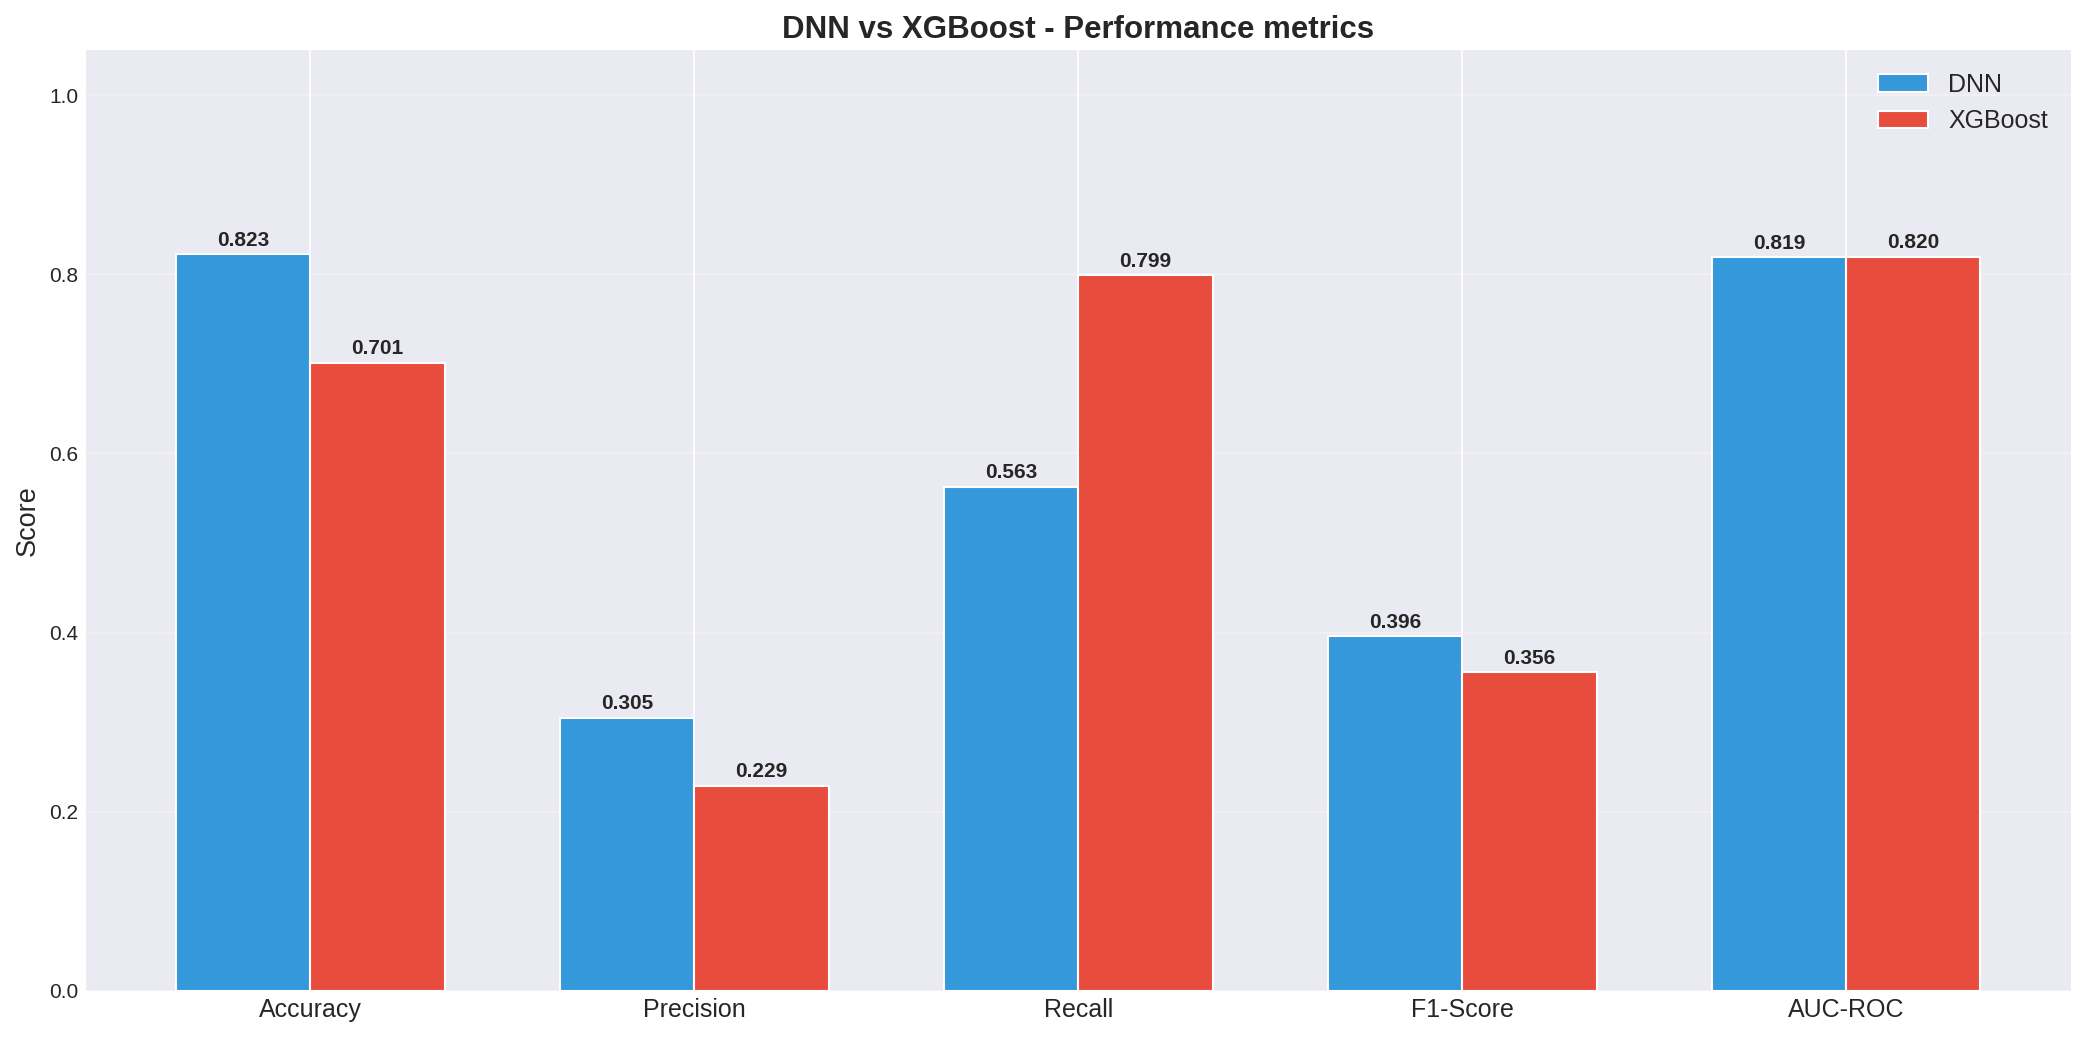
\includegraphics[width=\textwidth]{figures/metrics_comparison_barchart.png}
    \caption{Comparaison des métriques par histogramme pour DNN (seuil 0,5),
             DNN (seuil 0,67) et XGBoost. L'AUC-ROC converge vers 0,82 pour
             les trois modèles, tandis que le rappel et la précision varient
             selon le seuil choisi.}
    \label{fig:metrics_barchart}
\end{figure}

\begin{figure}[H]
    \centering
    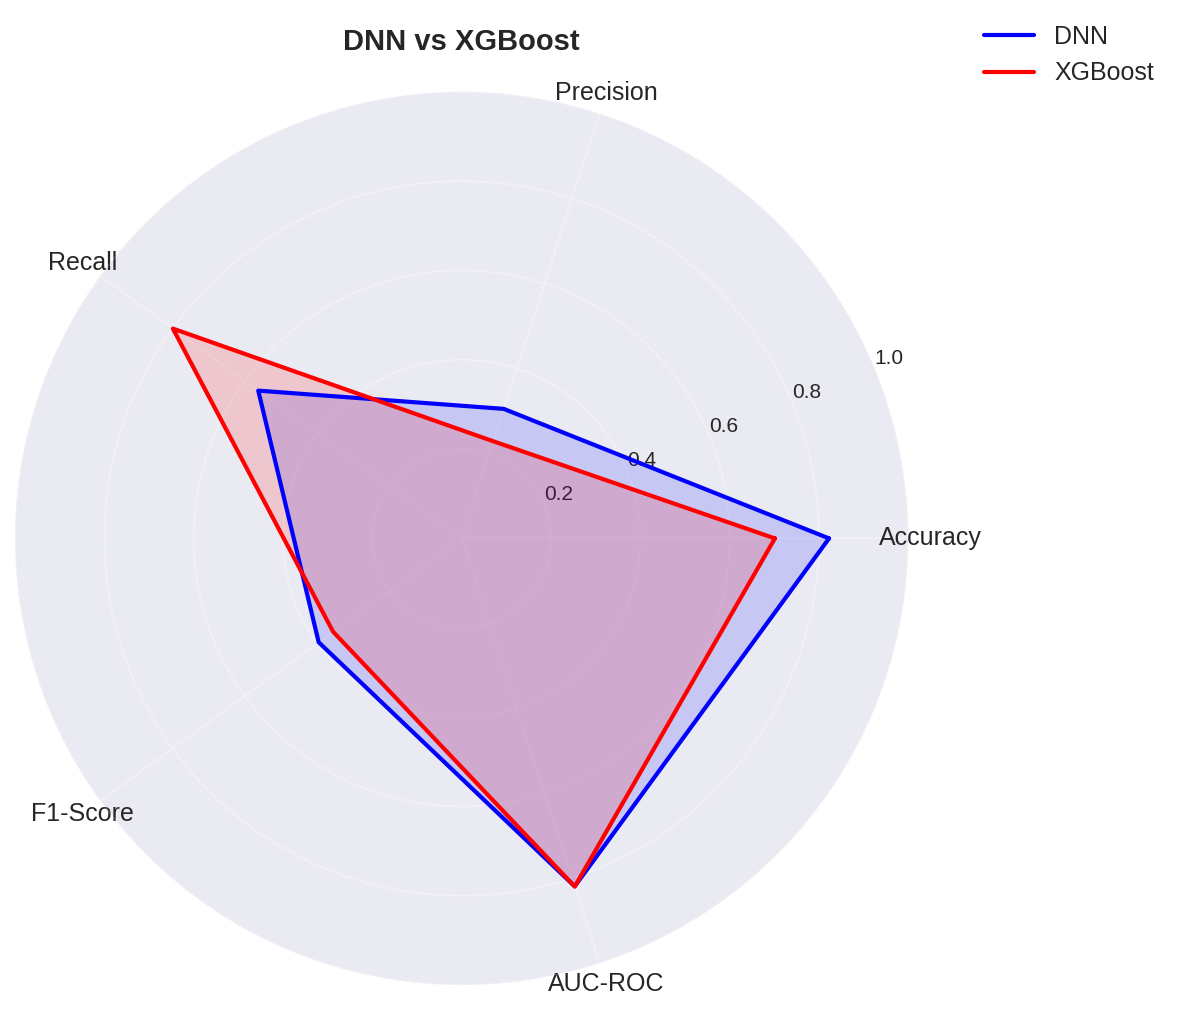
\includegraphics[width=0.70\textwidth]{figures/metrics_radar_chart.png}
    \caption{Graphique radar des métriques comparatives (accuracy, précision,
             rappel, F1-score, AUC-ROC). XGBoost au seuil 0,5 présente le
             meilleur rappel (79,9\%), tandis que DNN au seuil 0,67 offre
             le meilleur compromis précision-rappel (F1 = 0,396).}
    \label{fig:metrics_radar}
\end{figure}

\subsection{Résultats détaillés du DNN}

La figure~\ref{fig:dnn_roc} présente la courbe ROC du DNN, et la figure~\ref{fig:dnn_cm}
sa matrice de confusion au seuil optimal de 0,6713.

\begin{figure}[H]
    \centering
    \begin{subfigure}[b]{0.48\textwidth}
        \centering
        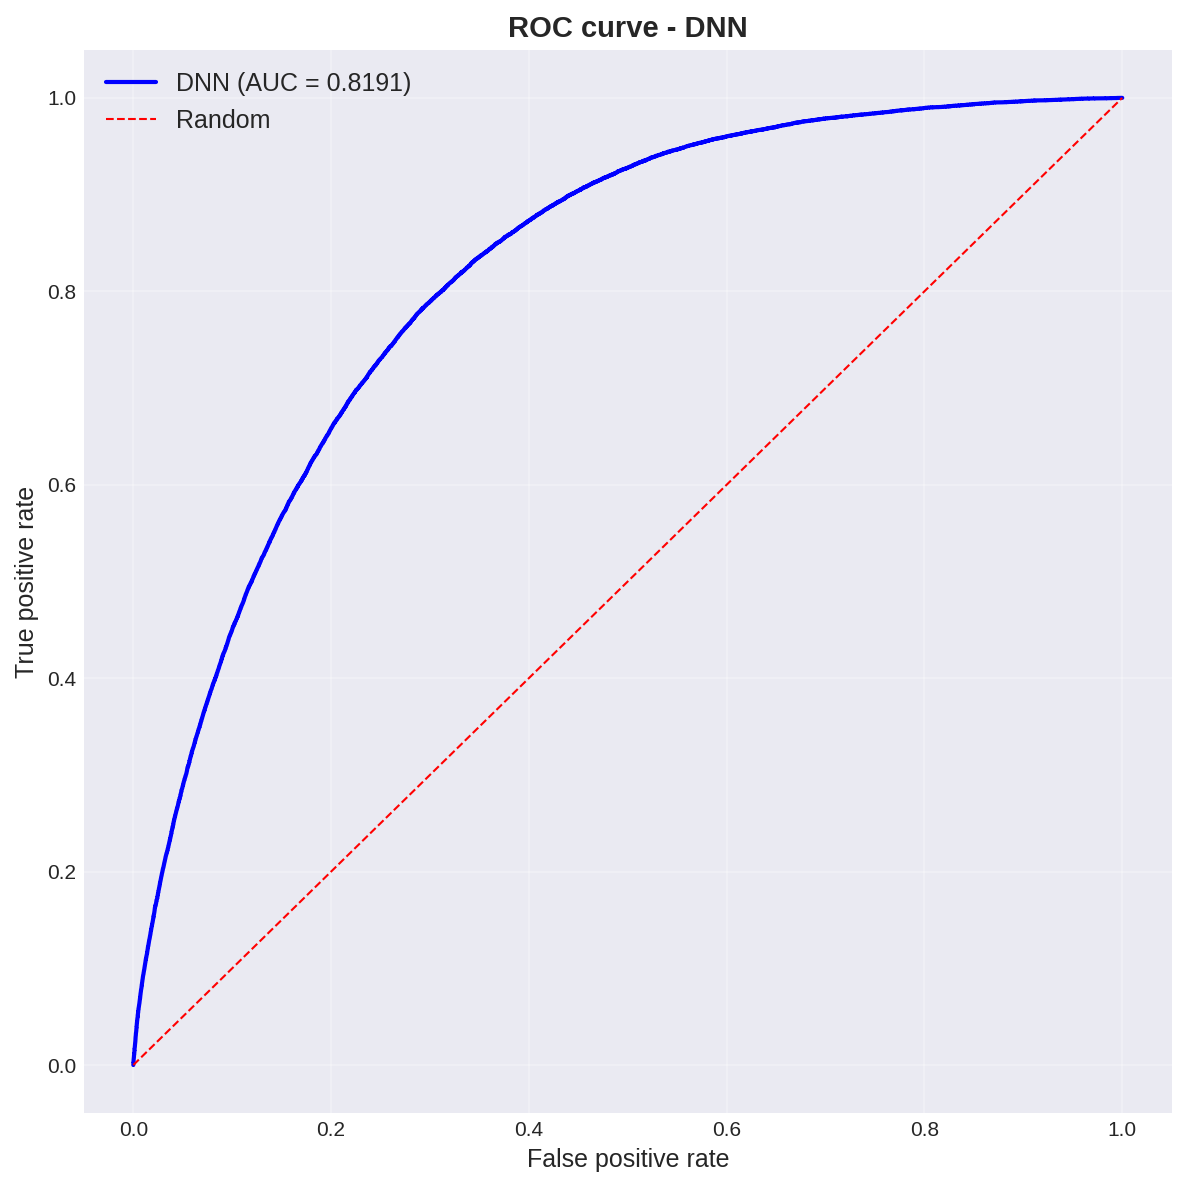
\includegraphics[width=\textwidth]{figures/dnn_roc_curve.png}
        \caption{Courbe ROC du DNN (AUC = 0,819)}
        \label{fig:dnn_roc}
    \end{subfigure}
    \hfill
    \begin{subfigure}[b]{0.48\textwidth}
        \centering
        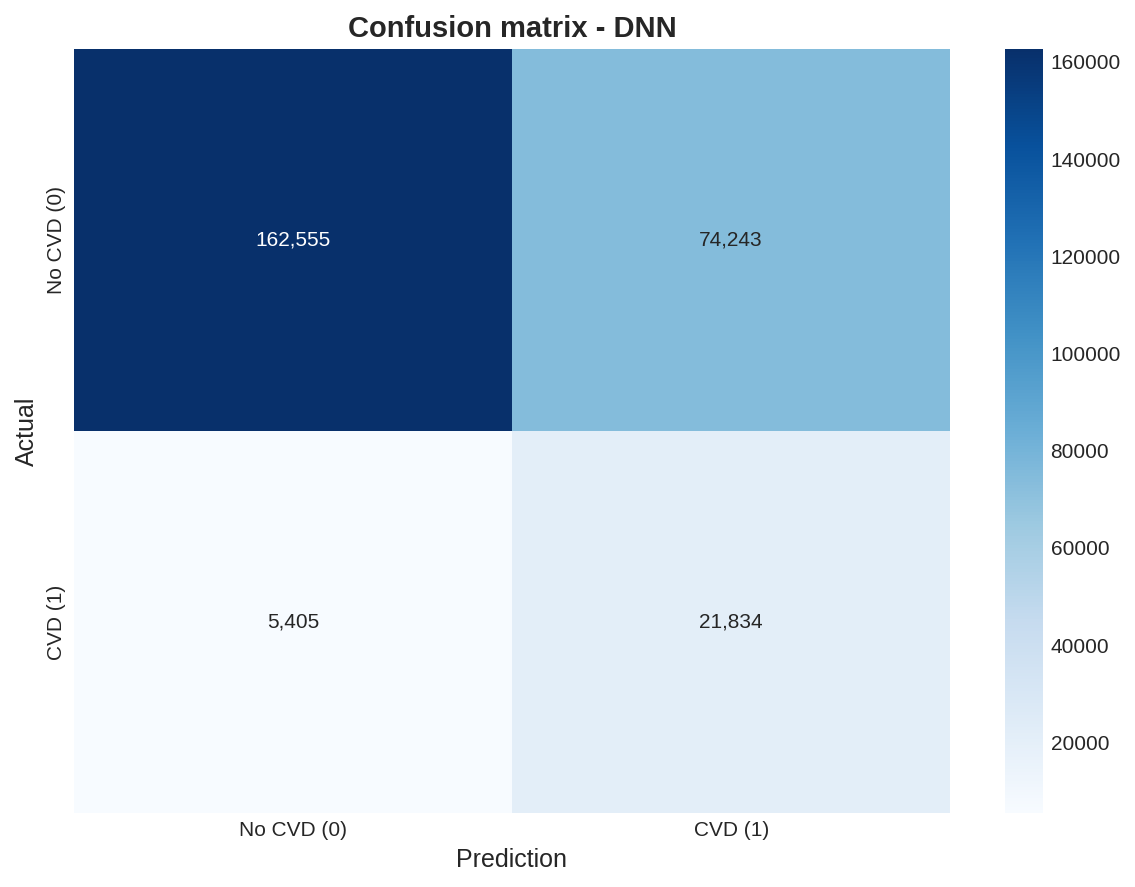
\includegraphics[width=\textwidth]{figures/dnn_confusion_matrix.png}
        \caption{Matrice de confusion (seuil 0,6713)}
        \label{fig:dnn_cm}
    \end{subfigure}
    \caption{Résultats du DNN~: courbe ROC et matrice de confusion au seuil optimal.
             15\,333 vrais positifs (patients MCV correctement identifiés)
             contre 11\,906 faux négatifs.}
    \label{fig:dnn_results}
\end{figure}

\subsection{Résultats détaillés d'XGBoost}

La figure~\ref{fig:xgb_results} présente la courbe ROC et la matrice de confusion
d'XGBoost au seuil par défaut 0,5.

\begin{figure}[H]
    \centering
    \begin{subfigure}[b]{0.48\textwidth}
        \centering
        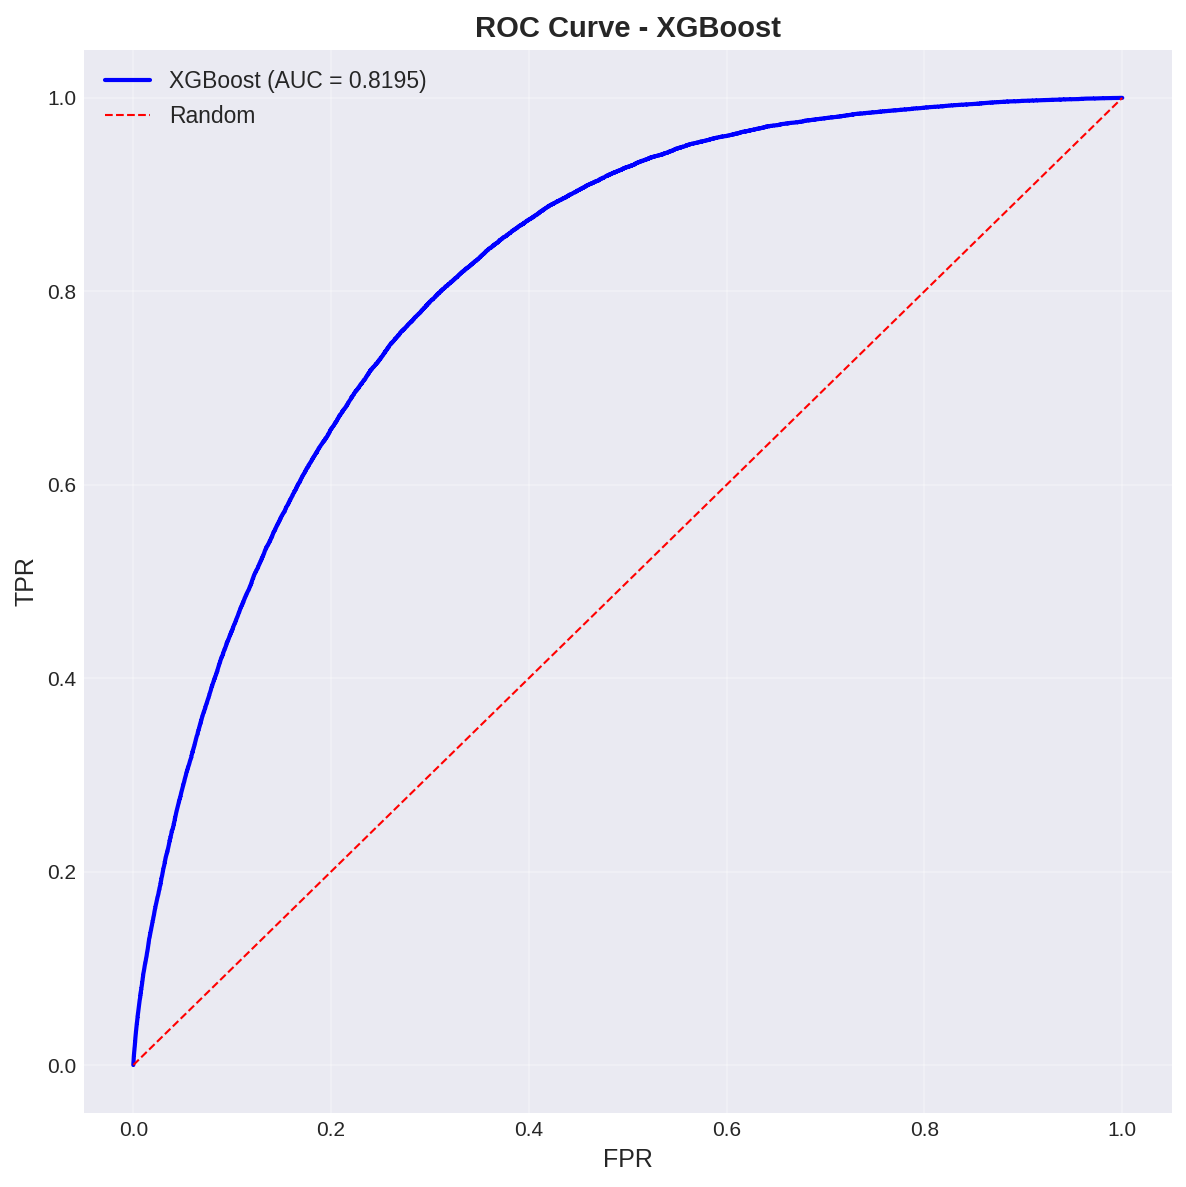
\includegraphics[width=\textwidth]{figures/xgboost_roc_curve.png}
        \caption{Courbe ROC XGBoost (AUC = 0,820)}
        \label{fig:xgb_roc}
    \end{subfigure}
    \hfill
    \begin{subfigure}[b]{0.48\textwidth}
        \centering
        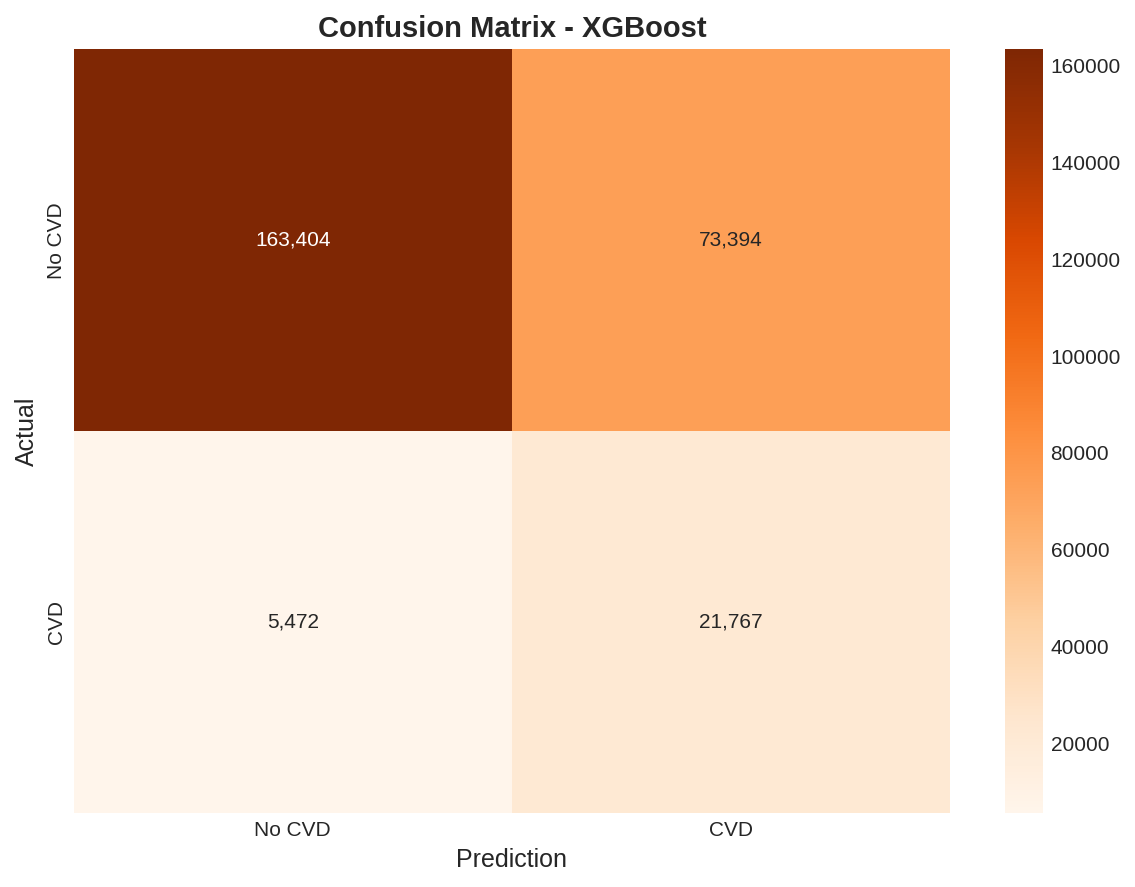
\includegraphics[width=\textwidth]{figures/xgboost_confusion_matrix.png}
        \caption{Matrice de confusion (seuil 0,5)}
        \label{fig:xgb_cm}
    \end{subfigure}
    \caption{Résultats XGBoost~: courbe ROC et matrice de confusion au seuil 0,5.
             21\,767 vrais positifs contre 5\,472 faux négatifs~; le rappel
             plus élevé (79,9\%) se fait au prix de 73\,394 faux positifs.}
    \label{fig:xgb_results}
\end{figure}

\subsection{Comparaison des courbes ROC}

La figure~\ref{fig:roc} superpose les courbes ROC des trois modèles.

\begin{figure}[H]
    \centering
    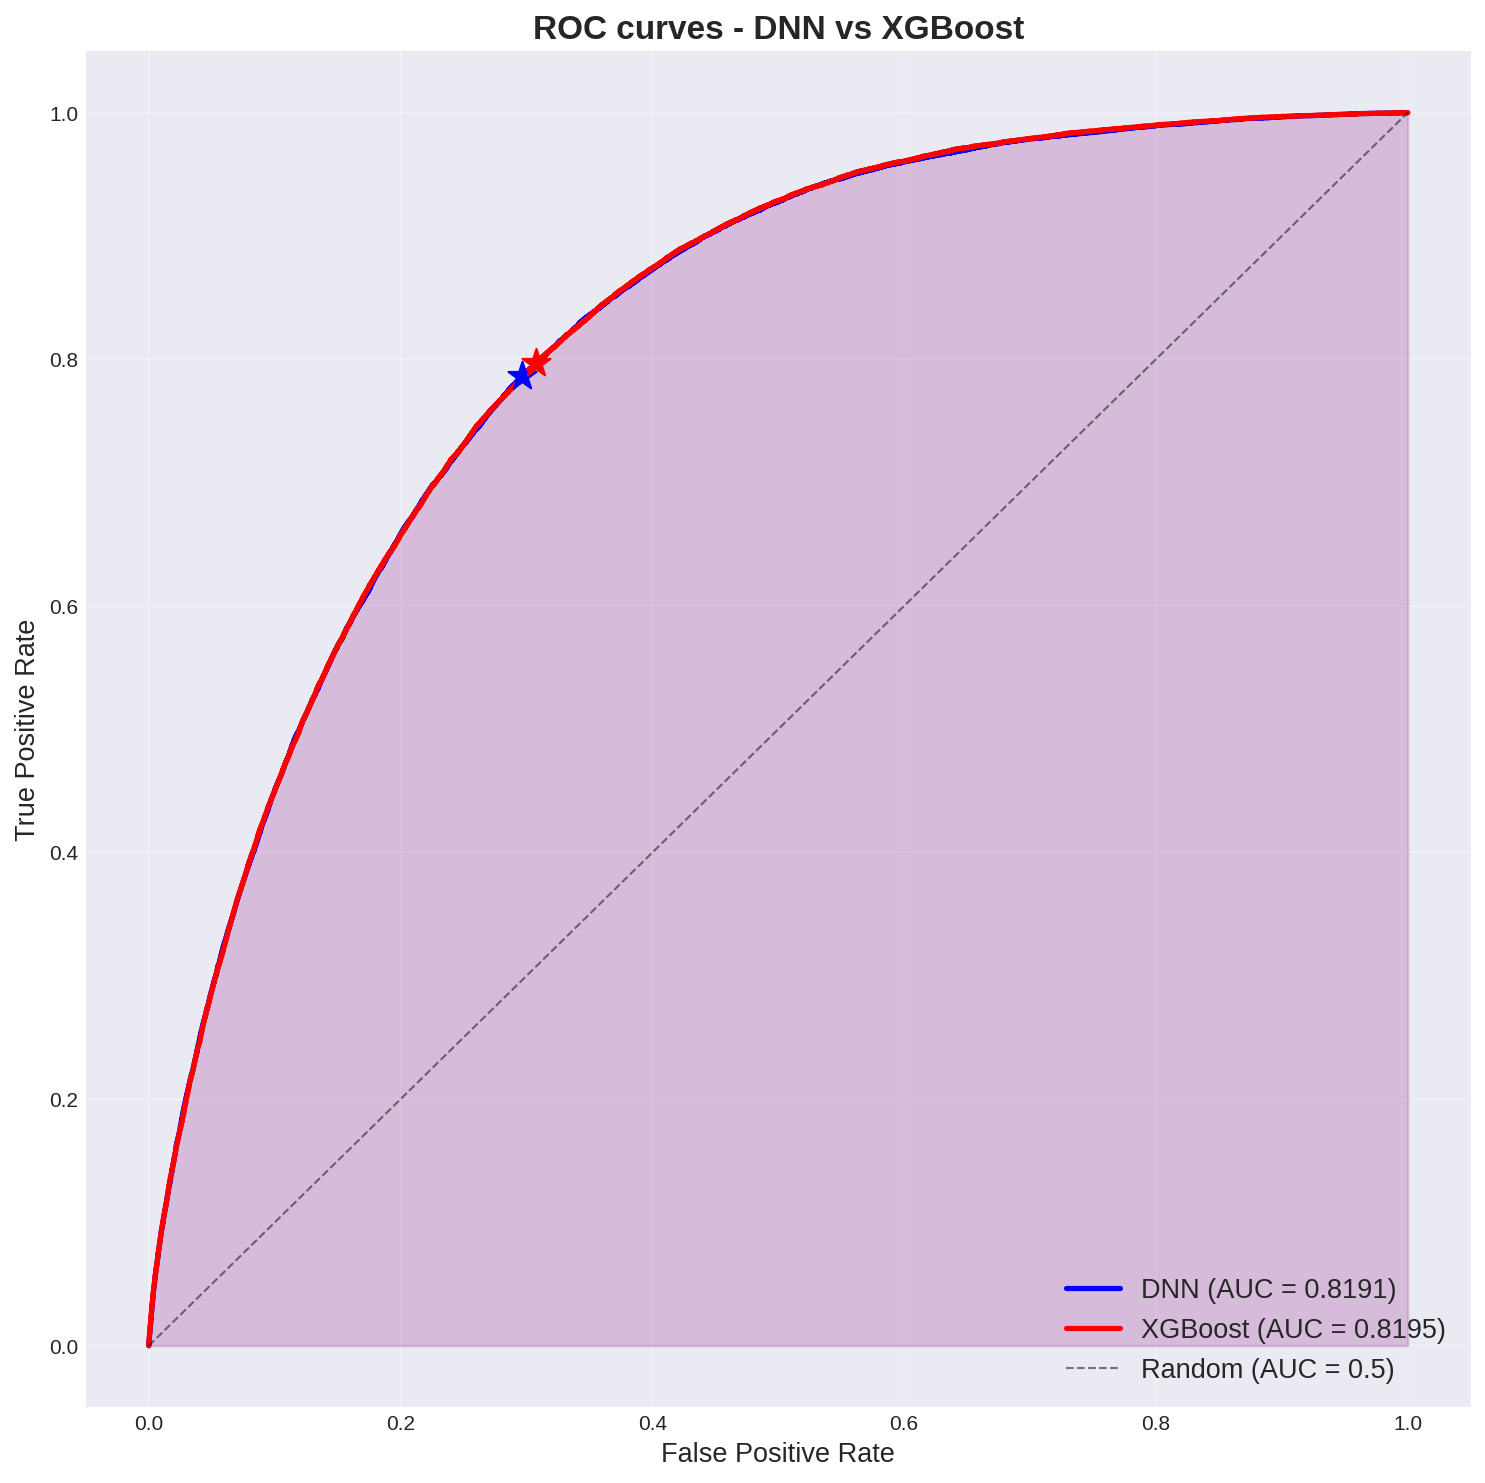
\includegraphics[width=0.85\textwidth]{figures/roc_curves.png}
    \caption{Courbes ROC superposées — DNN, XGBoost et Spark GBT. Les trois modèles
             convergent remarquablement vers le même AUC d'environ 0,82, indiquant
             un plateau déterminé par l'information disponible dans les features
             et non par les architectures des modèles.}
    \label{fig:roc}
\end{figure}

La convergence vers un AUC commun de 0,82 pour trois architectures fondamentalement
différentes (réseau de neurones profond, boosting de gradient, GBT distribué)
constitue une observation forte~: la limite de performance est imposée par
les données disponibles, et notamment par l'absence de \texttt{HighBP} et
\texttt{HighChol}, les deux variables les plus discriminantes selon la littérature.

\subsection{Matrices de confusion comparatives}

\begin{figure}[H]
    \centering
    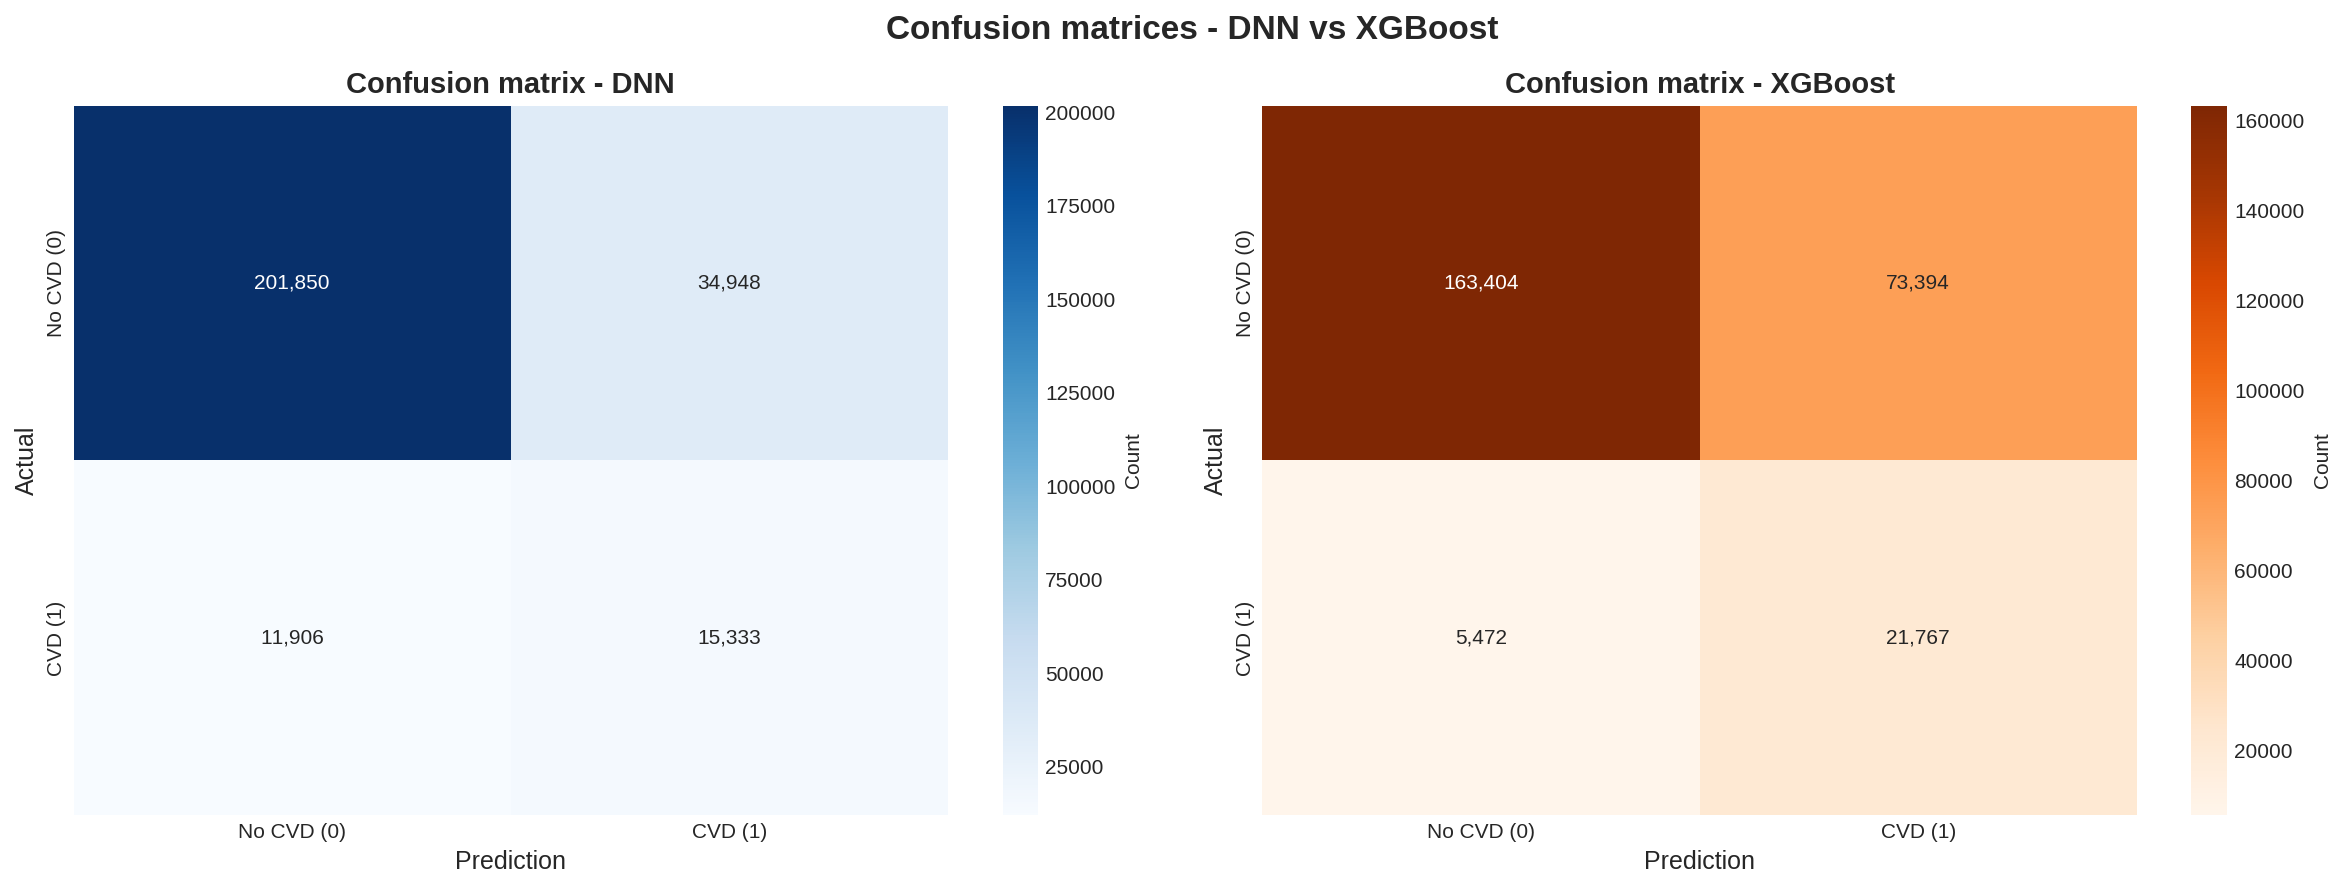
\includegraphics[width=\textwidth]{figures/confusion_matrices.png}
    \caption{Matrices de confusion comparatives — DNN (seuil 0,6713) et XGBoost
             (seuil 0,5). XGBoost présente moins de faux négatifs (5\,472 vs.
             11\,906) mais beaucoup plus de faux positifs (73\,394 vs. 34\,948).}
    \label{fig:cm}
\end{figure}

\begin{table}[H]
\centering
\caption{Analyse des matrices de confusion (jeu de test, 264\,037 observations)}
\label{tab:cm_analysis}
\begin{tabular}{lcccc}
\toprule
\textbf{Modèle} & \textbf{VP} & \textbf{FP} & \textbf{VN} & \textbf{FN} \\
\midrule
DNN (seuil 0,6713) & 15\,333 & 34\,948 & 201\,850 & 11\,906 \\
XGBoost (seuil 0,5) & 21\,767 & 73\,394 & 163\,404 &  5\,472 \\
\bottomrule
\end{tabular}
\end{table}

L'interprétation clinique de ce compromis est essentielle~:
\begin{itemize}
    \item \textbf{XGBoost} (rappel = 79,9\%)~: outil de dépistage précoce privilégiant
          la sensibilité — moins de patients MCV manqués, au prix d'un plus grand
          nombre de faux positifs nécessitant des examens complémentaires.
    \item \textbf{DNN (seuil 0,67)} (rappel = 56,3\%, précision = 30,5\%)~:
          outil de confirmation, réduisant les fausses alertes au détriment d'une
          plus grande proportion de MCV non détectées.
\end{itemize}

\subsection{Courbes d'apprentissage du DNN}

\begin{figure}[H]
    \centering
    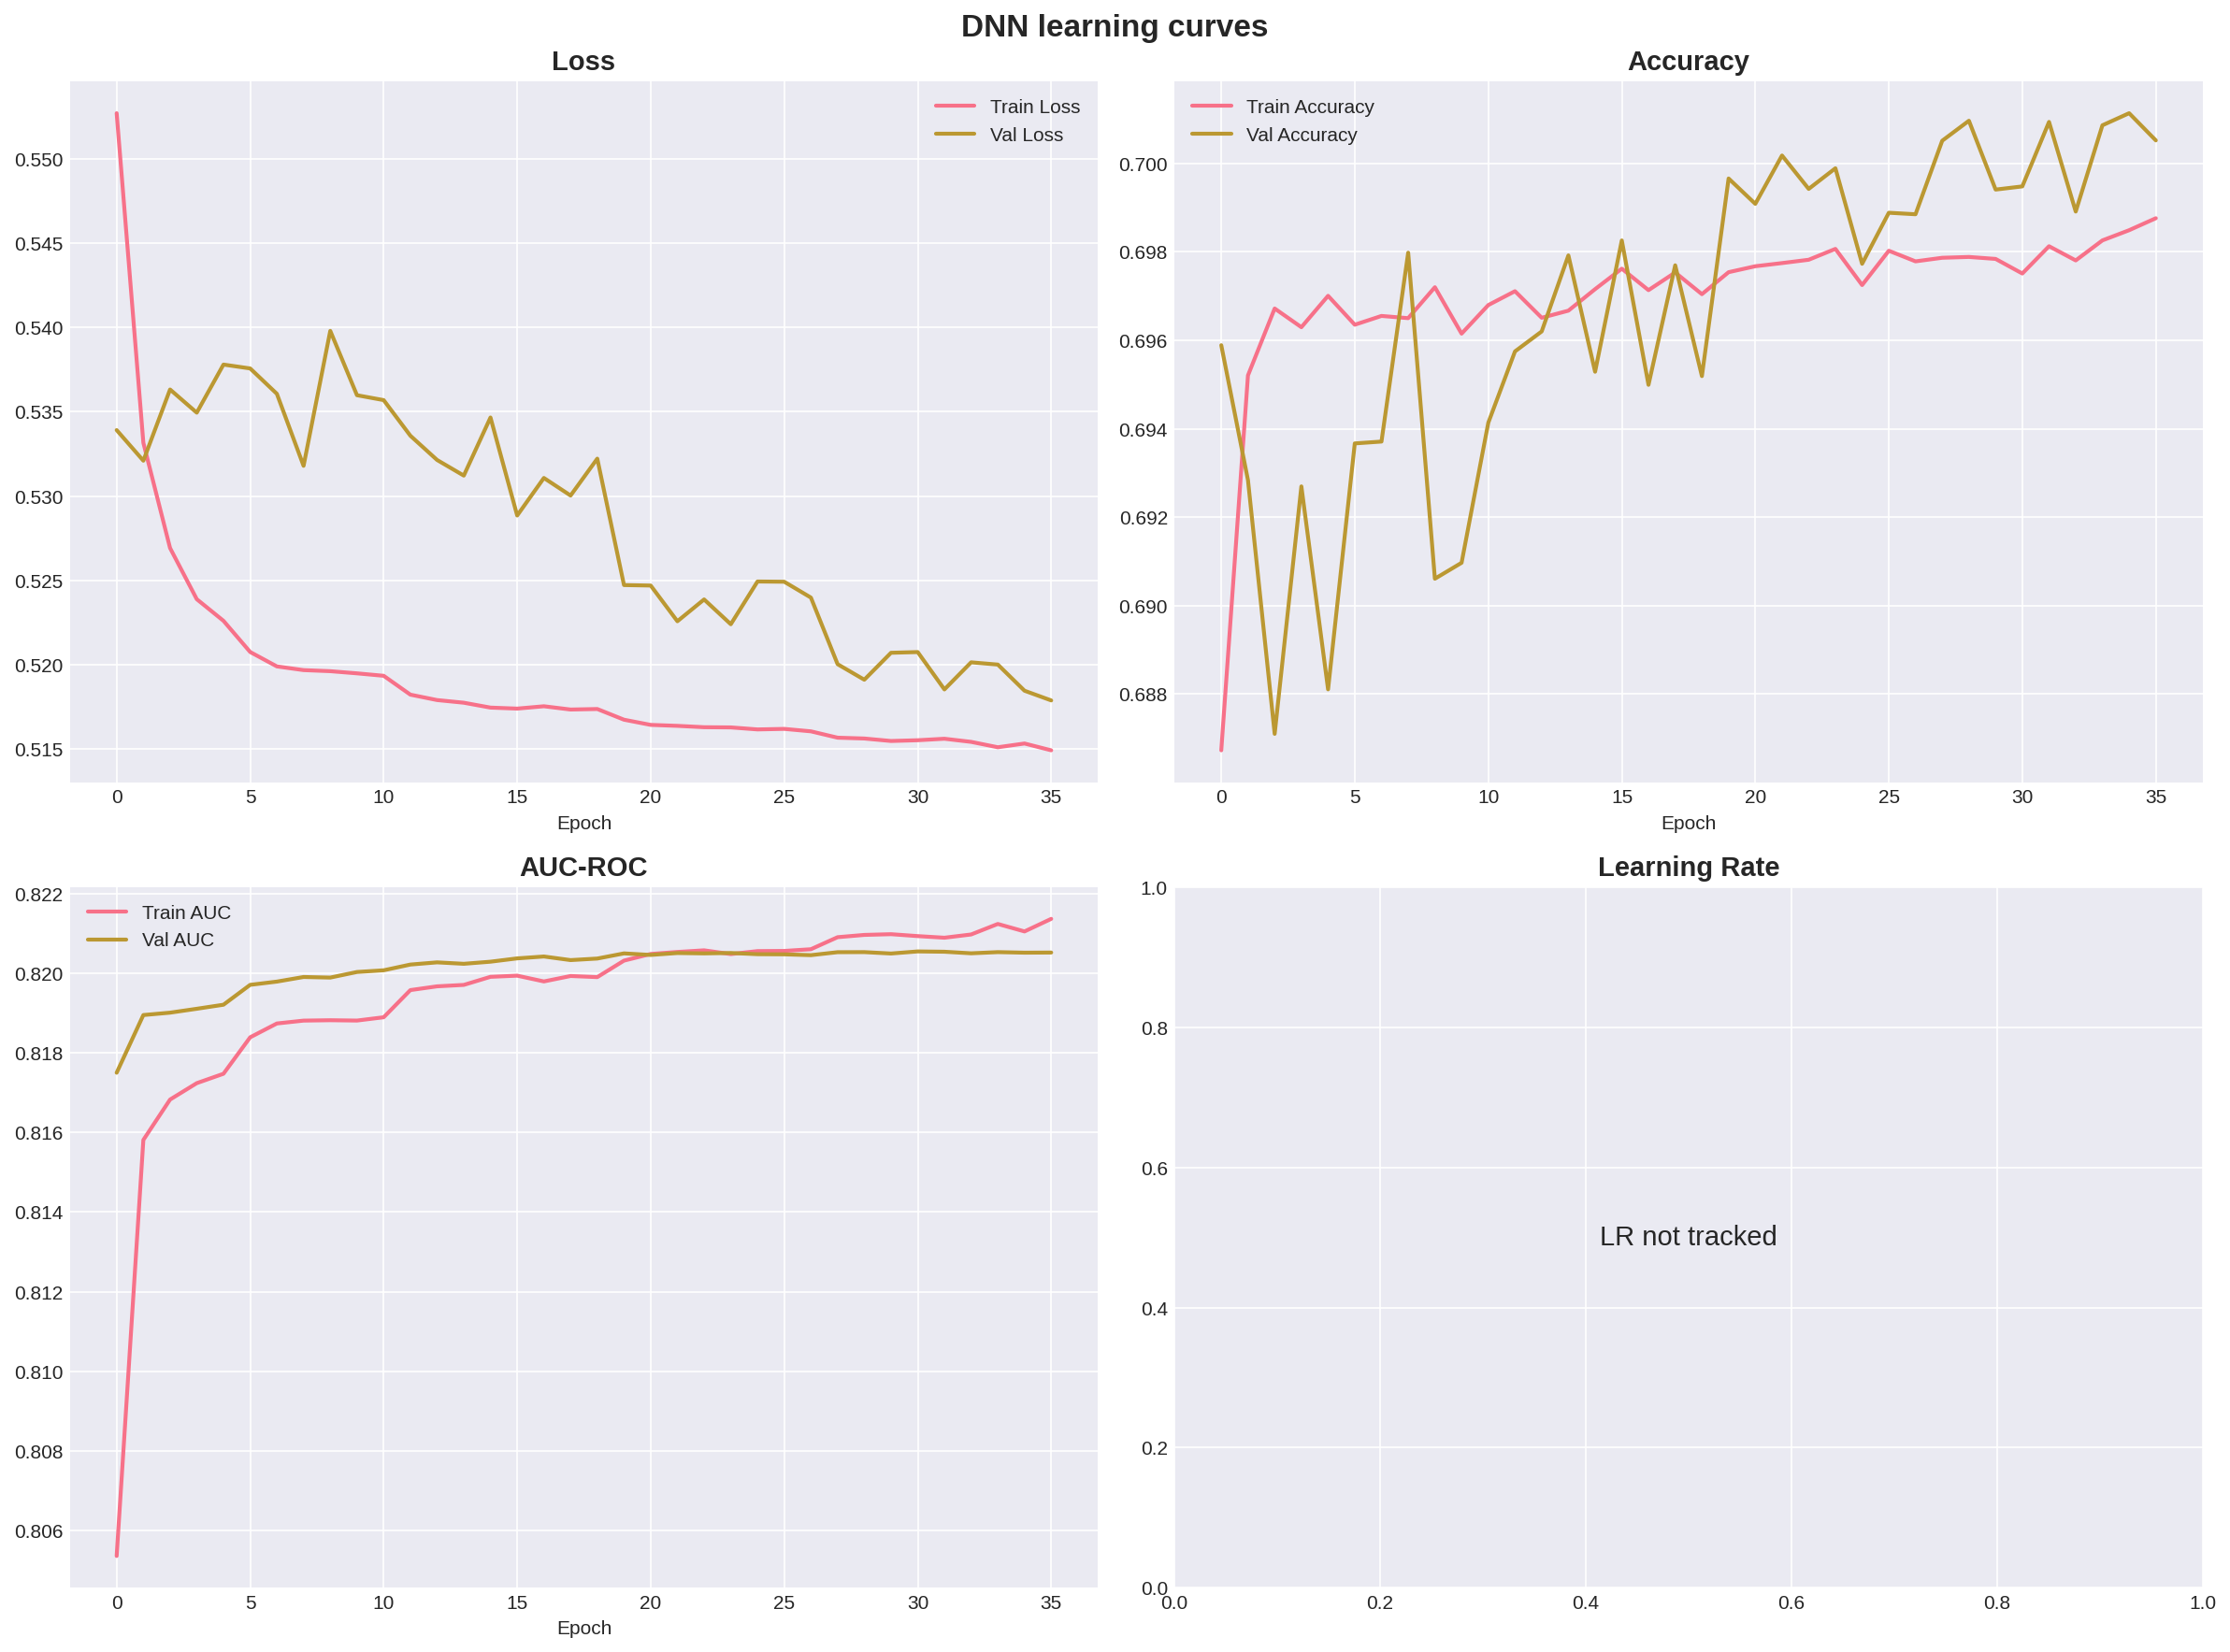
\includegraphics[width=0.85\textwidth]{figures/dnn_learning_curves.png}
    \caption{Courbes d'apprentissage du DNN — perte (gauche) et AUC (droite)
             sur les ensembles d'entraînement et de validation.
             L'AUC dépasse 0,82 dès l'epoch~1 et évolue faiblement
             (+0,003 sur 36 epochs), confirmant que le plateau est inhérent
             aux données et non à une capacité insuffisante du modèle.}
    \label{fig:lc}
\end{figure}

La convergence rapide et parallèle des courbes d'entraînement et de validation
(absence d'écart significatif) confirme l'absence de surapprentissage.
La combinaison Dropout (taux 0,30), BatchNormalization et régularisation $L_2$
($\lambda = 10^{-4}$) est efficace pour un jeu d'entraînement de 1,2~million
d'observations.

\subsection{Analyse du seuil de classification DNN}

\begin{figure}[H]
    \centering
    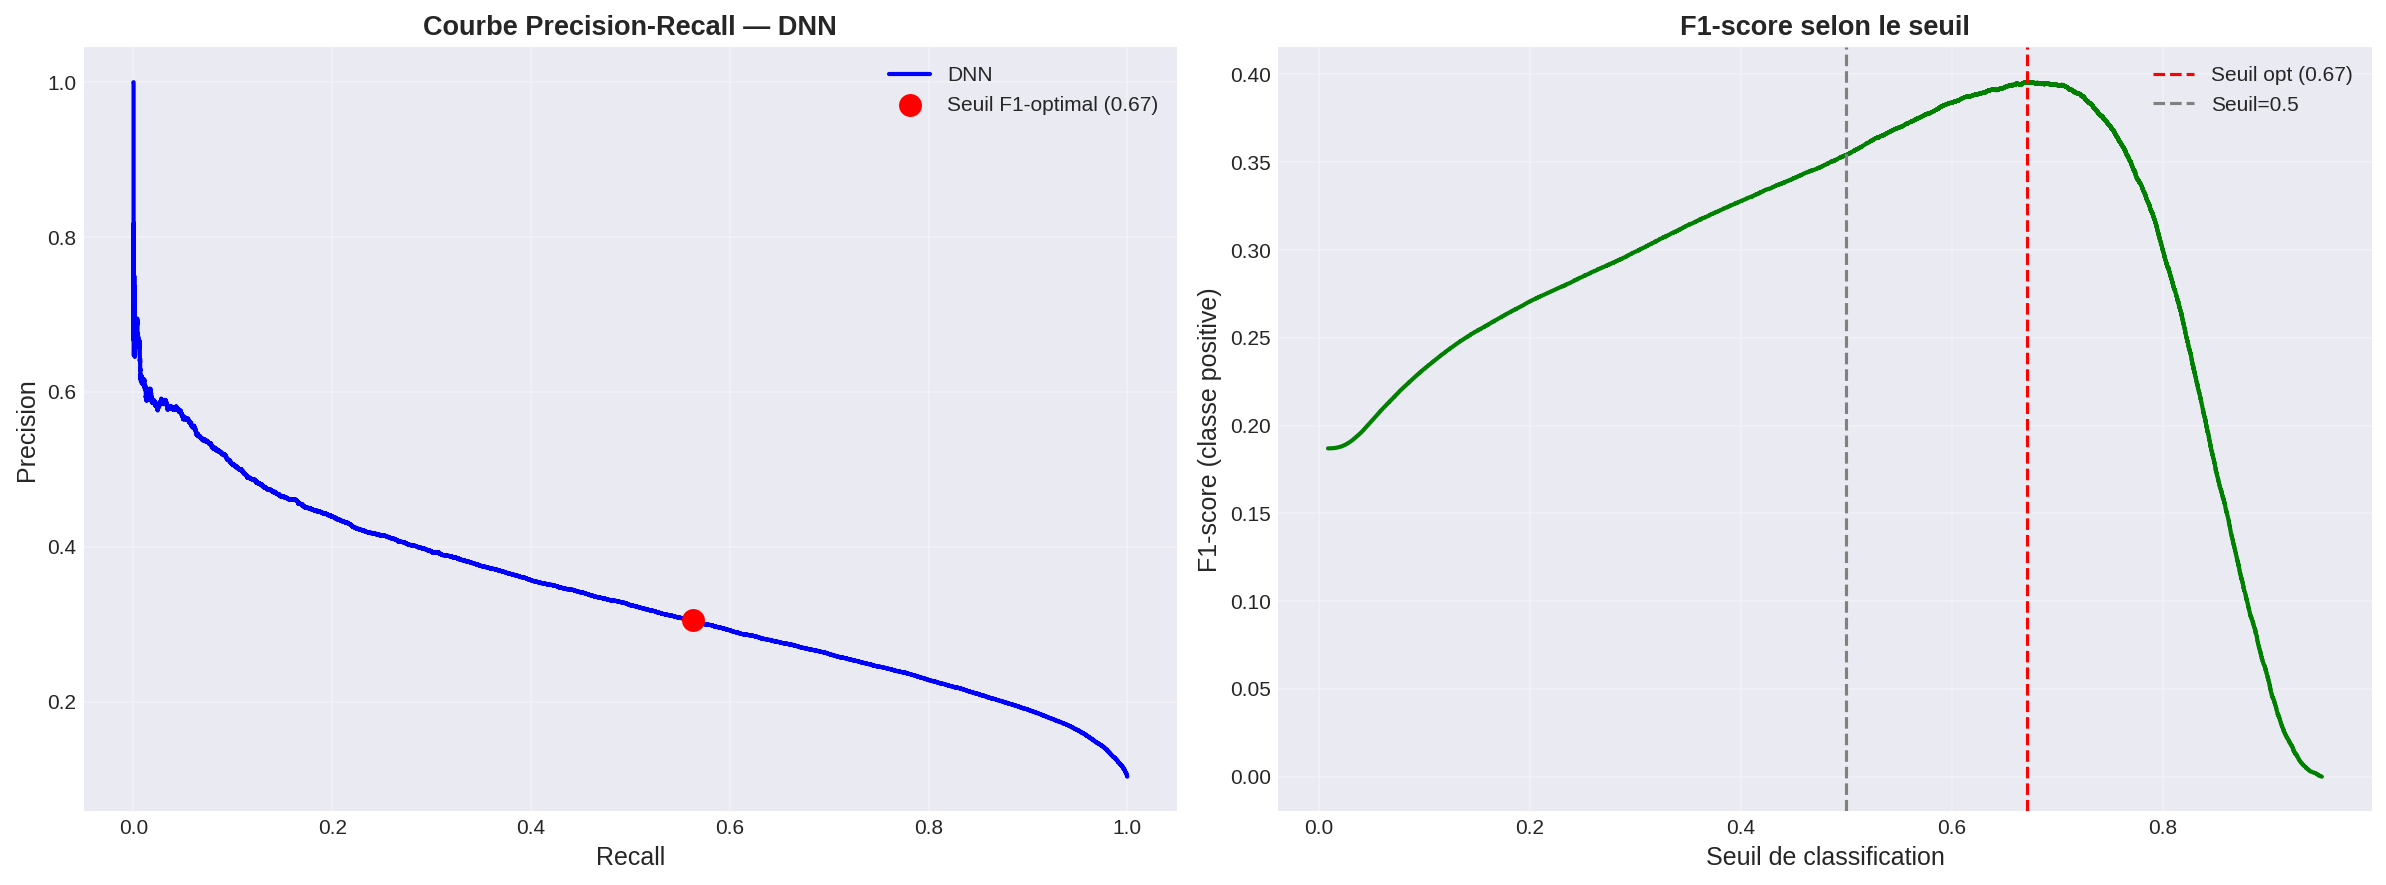
\includegraphics[width=0.85\textwidth]{figures/dnn_threshold_analysis.png}
    \caption{Courbe Précision-Rappel et F1-Score en fonction du seuil de
             classification. Le seuil optimal $\tau^* = 0{,}6713$ maximise le
             F1-score à 0,396. Le seuil par défaut 0,5 produit un rappel élevé
             (0,80) mais une précision très faible (0,23).}
    \label{fig:threshold}
\end{figure}

\begin{table}[H]
\centering
\caption{Impact du seuil de classification sur les métriques du DNN}
\label{tab:threshold_impact}
\begin{tabular}{lccc}
\toprule
\textbf{Seuil} & \textbf{Accuracy} & \textbf{Rappel} & \textbf{F1} \\
\midrule
0,50 (par défaut)       & 0,698 & 0,802 & 0,354 \\
0,6713 (F1-optimal) & 0,822 & 0,563 & 0,396 \\
\midrule
Gain relatif & +17,7\% & $-$29,8\% & +11,9\% \\
\bottomrule
\end{tabular}
\end{table}

L'optimisation du seuil améliore le F1-score de 11,9\% en acceptant une réduction
de 29,8\% du rappel. Ce compromis met en évidence l'importance du choix du seuil
dans les applications cliniques : il n'existe pas de seuil universellement optimal,
et la décision doit être guidée par les coûts relatifs des faux positifs et des
faux négatifs dans le contexte clinique visé.

\subsection{Importance des features XGBoost}

\begin{figure}[H]
    \centering
    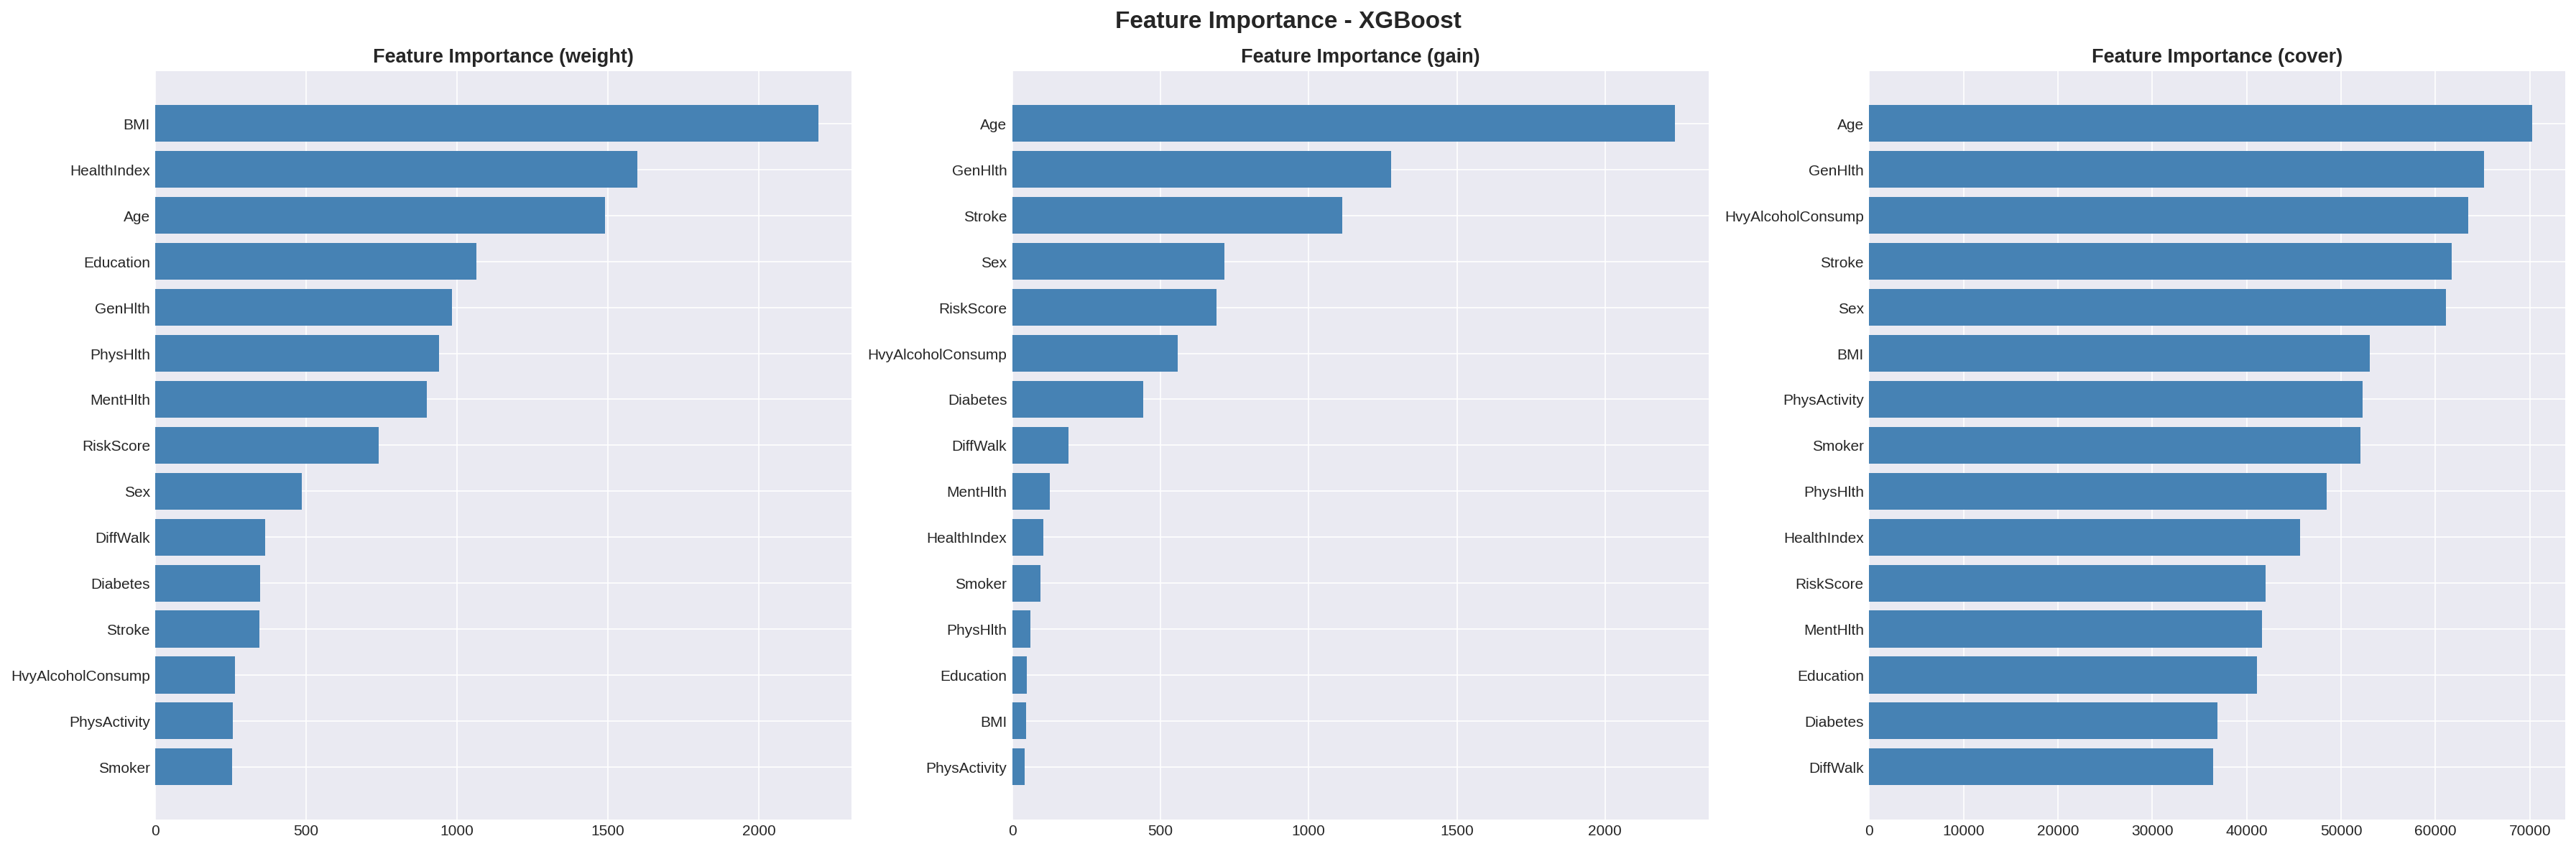
\includegraphics[width=0.85\textwidth]{figures/xgboost_feature_importance.png}
    \caption{Importance des features XGBoost selon trois critères~:
             \textit{weight} (fréquence de coupure), \textit{gain}
             (gain d'information moyen par coupure) et \textit{cover}
             (fraction d'observations affectées). Le critère \textit{gain}
             est le plus informatif~: Age, GenHlth et Stroke dominent,
             en concordance avec l'importance Gini du Random Forest préliminaire.}
    \label{fig:xgb_fi}
\end{figure}

Le critère \textit{weight} place BMI en tête~: sa grande plage de valeurs distinctes
(variable continue) génère naturellement un plus grand nombre de points de coupure
utilisés, sans que cela reflète une importance prédictive supérieure.
Ce biais de fréquence, bien documenté pour les variables continues dans XGBoost,
explique la divergence avec le critère \textit{gain}, qui reste la référence
pour comparer l'importance effective des features.

% ─────────────────────────────────────────────────────────────────────────────
\section{Impact d'Apache Spark}
% ─────────────────────────────────────────────────────────────────────────────

\subsection{Benchmark temporel Spark vs. XGBoost standalone}

La figure~\ref{fig:benchmark} présente les temps d'entraînement comparatifs
entre XGBoost standalone et Spark GBTClassifier pour cinq fractions croissantes
du jeu de données.

\begin{figure}[H]
    \centering
    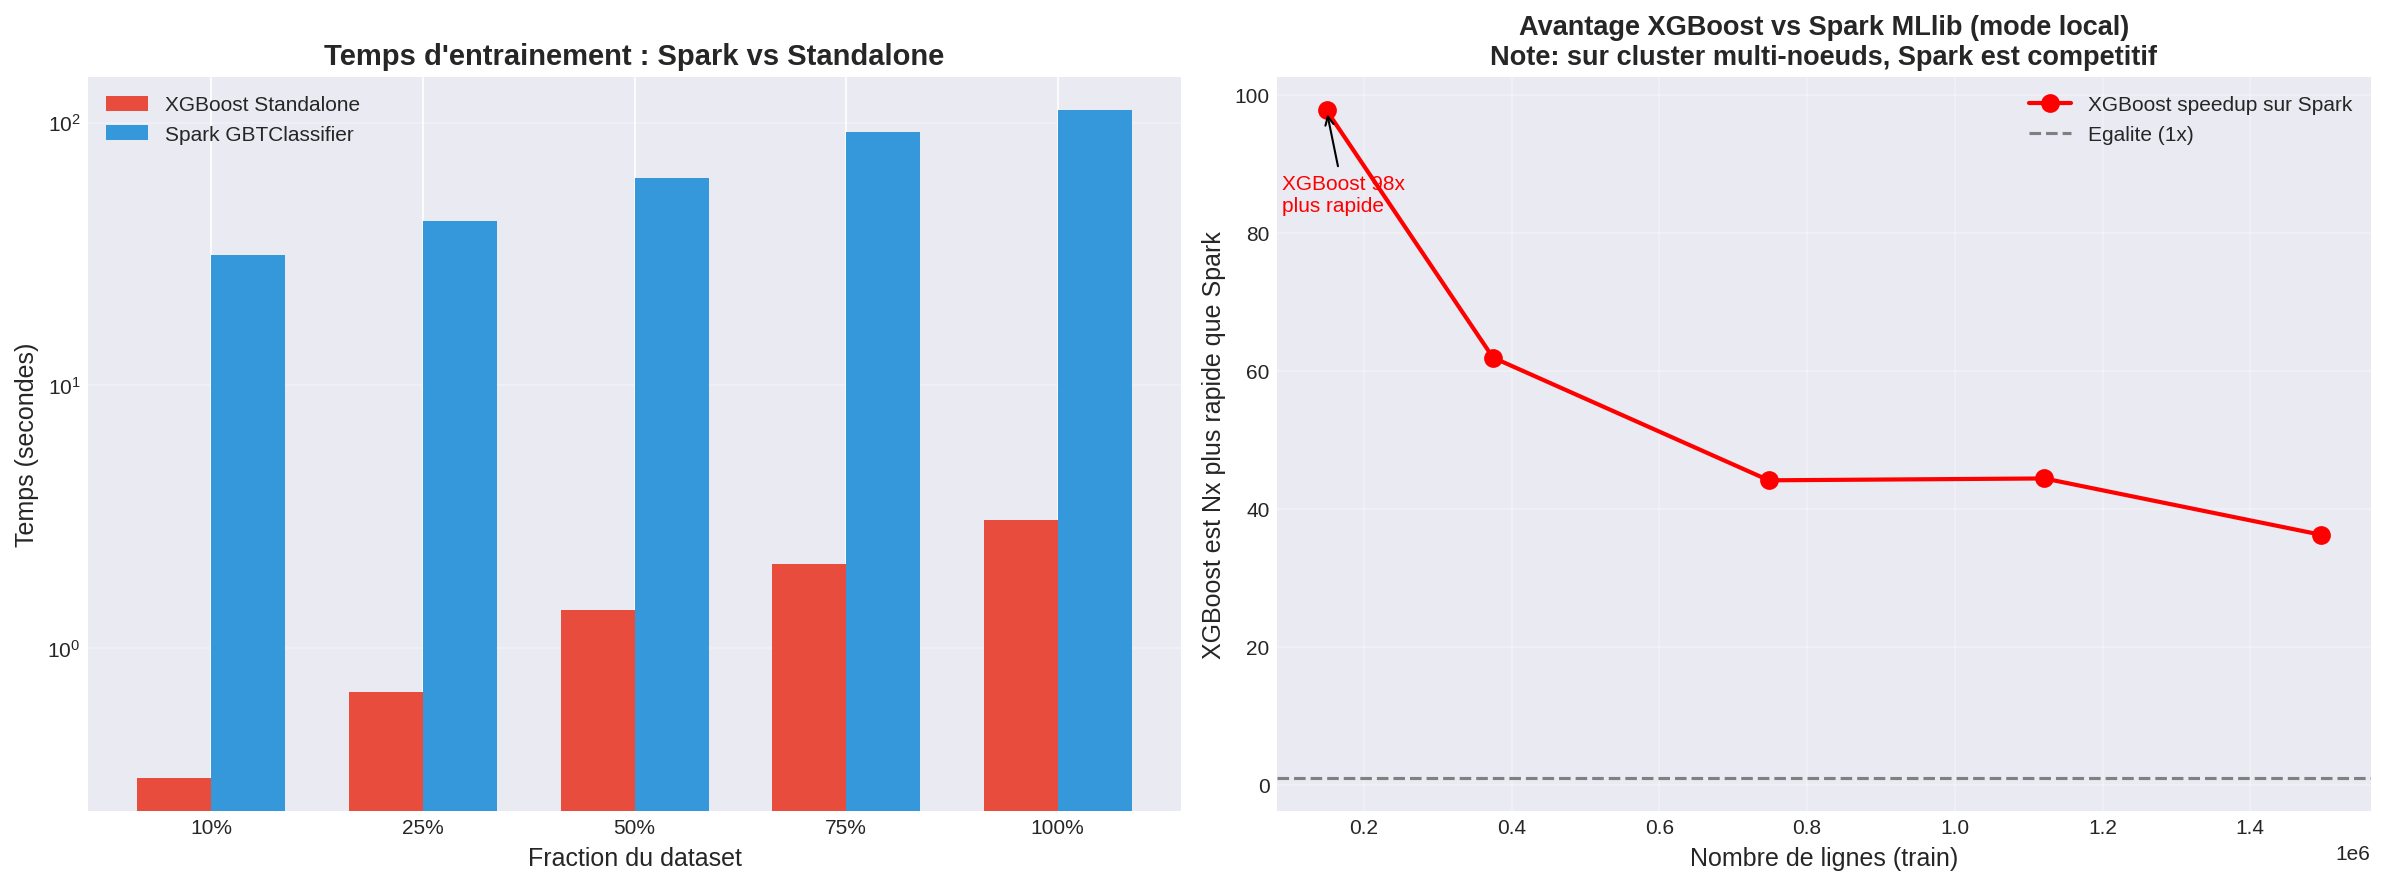
\includegraphics[width=\textwidth]{figures/spark_benchmark_comparison.png}
    \caption{Benchmark temps d'entraînement --- Spark GBT vs XGBoost standalone
             sur cinq fractions du jeu de données (10\% à 100\%).
             L'avantage XGBoost est maximal pour les petits volumes (97,7$\times$
             à 150\,000 lignes) et se réduit à 36$\times$ pour le volume complet.}
    \label{fig:benchmark}
\end{figure}

\begin{table}[H]
\centering
\caption{Résultats détaillés du benchmark (mode local, Kaggle T4 $\times$2)}
\label{tab:benchmark}
\begin{tabular}{lrrrr}
\toprule
\textbf{Fraction} & \textbf{N lignes} & \textbf{Spark GBT (s)} & \textbf{XGBoost (s)} & \textbf{Avantage XGB} \\
\midrule
10\%  &    149\,510 &  31,23 &  0,32 & $\mathbf{97{,}7\times}$ \\
25\%  &    374\,916 &  42,07 &  0,68 & $\mathbf{61{,}9\times}$ \\
50\%  &    748\,199 &  61,41 &  1,39 & $\mathbf{44{,}2\times}$ \\
75\%  &  1\,121\,242 &  92,24 &  2,08 & $\mathbf{44{,}3\times}$ \\
100\% &  1\,495\,609 & 111,35 &  3,07 & $\mathbf{36{,}2\times}$ \\
\bottomrule
\end{tabular}
\end{table}

\subsection{Comparaison globale des temps d'exécution}

La figure~\ref{fig:timing} compare les temps d'entraînement et d'inférence
des trois modèles finaux (DNN, XGBoost avec RandomizedSearchCV, Spark GBT)
dans leur configuration complète.

\begin{figure}[H]
    \centering
    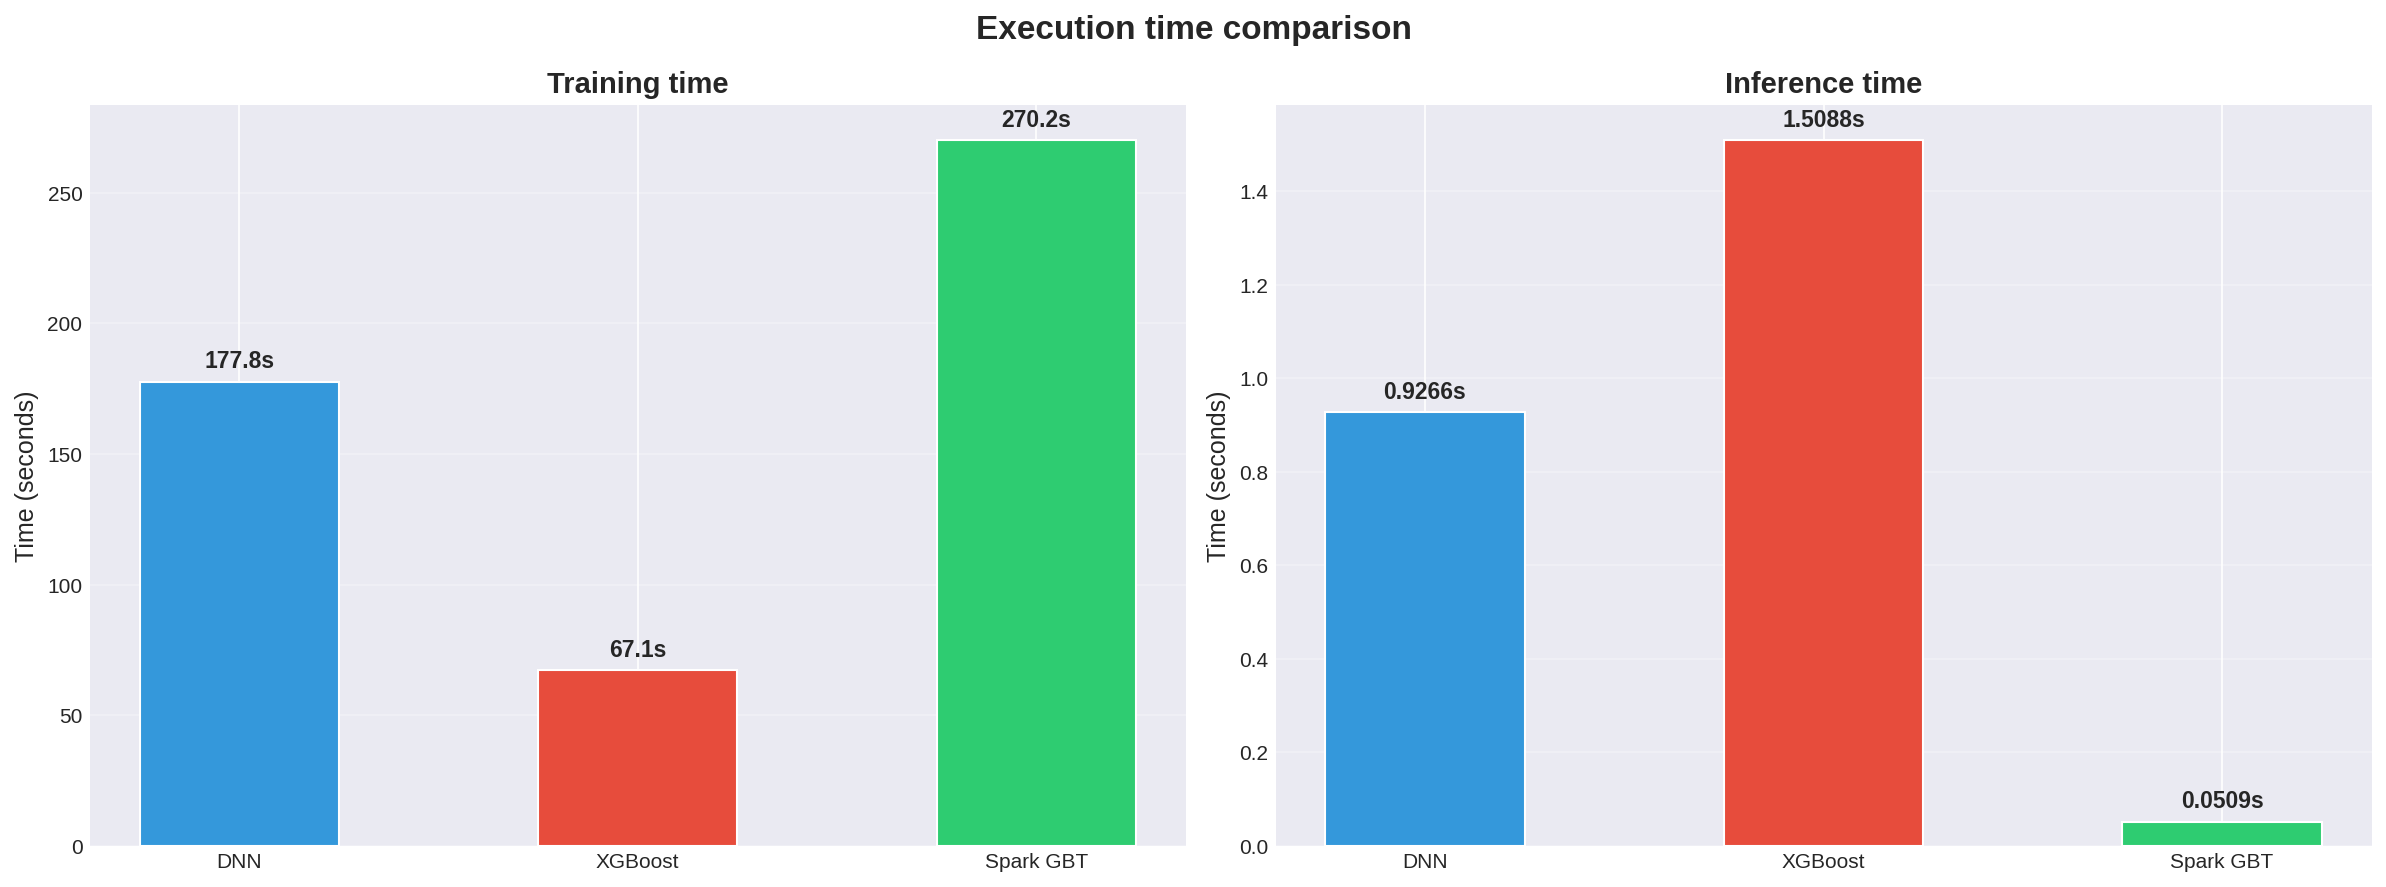
\includegraphics[width=\textwidth]{figures/timing_comparison.png}
    \caption{Comparaison des temps d'entraînement et d'inférence des trois modèles.
             XGBoost (67,1~s d'entraînement, 1,5~s d'inférence) offre le meilleur
             rapport performance/coût computationnel.
             Spark GBT (270,2~s) est le plus lent en mode local~;
             le DNN (177,8~s) bénéficie de l'accélération GPU.}
    \label{fig:timing}
\end{figure}

\textbf{Observations principales~:}
\begin{enumerate}
    \item XGBoost est \textbf{36 à 97 fois plus rapide} que Spark GBT en mode local.
          Cet écart est maximal pour les petits volumes (97,7$\times$ à 150\,000 lignes)
          et se réduit à mesure que le volume augmente, reflétant l'amortissement
          progressif de l'overhead fixe du scheduler Spark.
    \item Le temps Spark croît de façon quasi-linéaire (31~s $\to$ 111~s pour 10$\times$
          plus de données), ce qui traduit l'overhead constant du scheduler par partition.
    \item Le temps XGBoost croît de façon sous-linéaire (0,32~s $\to$ 3,07~s),
          bénéficiant de la parallélisation native C++/CUDA.
\end{enumerate}

\subsection{Apport réel de Spark dans ce pipeline}

Bien que Spark GBTClassifier soit systématiquement plus lent qu'XGBoost en mode
local, Apache Spark apporte une valeur ajoutée indispensable dans les phases de
preprocessing~:

\begin{itemize}
    \item Lecture et déduplication de 2,17~millions de lignes Parquet en quelques
          secondes~; cette opération bloquerait un DataFrame pandas sur 29~Go de RAM.
    \item Calcul parallèle des statistiques descriptives sur l'ensemble du dataset
          distribué.
    \item Scalabilité~: sur un cluster HDFS/YARN de 8~nœuds ou plus, Spark
          deviendrait compétitif pour des volumes dépassant 10~millions de lignes,
          conformément aux résultats de Zhang et al.~\cite{zhang2023}.
\end{itemize}

% ─────────────────────────────────────────────────────────────────────────────
\section{Vérification des critères de succès (PRD)}
% ─────────────────────────────────────────────────────────────────────────────

\begin{table}[H]
\centering
\caption{Vérification des critères de succès du PRD}
\label{tab:prd_check}
\begin{tabular}{llll}
\toprule
\textbf{Critère} & \textbf{Cible PRD} & \textbf{Résultat} & \textbf{Statut} \\
\midrule
AUC-ROC DNN      & $\geq 0{,}85$ & 0,819 & \textcolor{red}{$\times$ Non atteint} \\
AUC-ROC XGBoost  & $\geq 0{,}87$ & 0,820 & \textcolor{red}{$\times$ Non atteint} \\
F1 classe positive & $\geq 0{,}60$ & 0,396 (DNN, seuil opt.) & \textcolor{red}{$\times$ Non atteint} \\
Recall classe positive & $\geq 0{,}65$ & 0,799 (XGBoost) & \textcolor{green!60!black}{$\checkmark$ Atteint} \\
Pipeline Spark fonctionnel & --- & Oui & \textcolor{green!60!black}{$\checkmark$ Atteint} \\
Dashboard Streamlit & --- & Oui & \textcolor{green!60!black}{$\checkmark$ Atteint} \\
\bottomrule
\end{tabular}
\end{table}

\textbf{Analyse des écarts~:} Les cibles AUC de 0,85 (DNN) et 0,87 (XGBoost)
proviennent de la littérature utilisant des datasets BRFSS incluant \texttt{HighBP}
et \texttt{HighChol}, les deux variables les plus discriminantes.
L'absence de ces variables dans notre fichier poolé ML explique structurellement
un écart de 0,03 à 0,05 en AUC. Cette contrainte est d'ordre documentaire~:
avec les mêmes features, les modèles seraient attendus à des performances comparables
à celles de la littérature.

% ─────────────────────────────────────────────────────────────────────────────
\section{Discussion}
\label{sec:discussion}
% ─────────────────────────────────────────────────────────────────────────────

\subsection{Comparaison avec la littérature}

Le tableau~\ref{tab:etat_art_rappel} repositionne les résultats obtenus dans
le panorama des travaux comparables.

\begin{table}[H]
\centering
\caption{Positionnement des résultats dans la littérature}
\label{tab:etat_art_rappel}
\begin{tabular}{p{3.5cm}p{1.5cm}p{3cm}p{1.5cm}p{3.5cm}}
\toprule
\textbf{Auteurs} & \textbf{Année} & \textbf{Méthode} & \textbf{AUC} & \textbf{Particularités} \\
\midrule
Nickels et al.~\cite{nickels2023}    & 2023 & Random Forest       & 0,912 & Avec HighBP/HighChol \\
Mesdaghinia et al.~\cite{mesdaghinia2023} & 2023 & XGBoost + SMOTE & 0,872 & 23 variables \\
Kumar et al.~\cite{kumar2023}        & 2023 & LSTM                & 0,891 & Données longitudinales \\
Patel et al.~\cite{patel2023}        & 2023 & DNN + SMOTE         & 0,834 & F1=0,834 \\
\midrule
\textbf{Ce travail}                  & 2026 & DNN + XGBoost + Spark & 0,820 & Sans HighBP/HighChol \\
\bottomrule
\end{tabular}
\end{table}

Notre AUC de 0,819--0,820 se positionne de façon cohérente dans la littérature,
compte tenu des contraintes de features. Sans \texttt{HighBP} et \texttt{HighChol},
les performances typiques des travaux BRFSS se situent entre 0,80 et 0,85~;
notre résultat est donc proche de la limite supérieure atteignable avec le jeu
de données disponible.

\subsection{Convergence des modèles}

La convergence remarquable des trois modèles vers le même AUC de 0,82 représente
un résultat théoriquement significatif~: elle suggère l'existence d'un plafond
informationnel déterminé par les features disponibles, indépendamment de
l'architecture du classifieur. Ce phénomène est cohérent avec la théorie de
l'information~: lorsque les features ne contiennent pas suffisamment d'information
pour discriminer les classes, aucune architecture ne peut compenser ce déficit.

\subsection{Gestion du déséquilibre de classes}

La stratégie de pondération de classes s'avère efficace~: le Recall de la classe
positive atteint 79,9\% pour XGBoost (seuil 0,5), ce qui est cliniquement
satisfaisant pour un outil de dépistage précoce. Par rapport à SMOTE \cite{chawla2002smote},
la pondération préserve les distributions statistiques originales, essentielles
pour l'interprétabilité épidémiologique des résultats.

\subsection{Limites de l'étude}

\begin{enumerate}
    \item \textbf{Features manquantes}~: \texttt{HighBP}, \texttt{HighChol},
          \texttt{Income} et \texttt{NoDocbcCost} sont absentes du fichier poolé ML
          disponible, plafonnant la performance maximale atteignable à environ 0,82 en AUC.

    \item \textbf{Mode local Spark}~: L'évaluation de Spark en mode local (une seule
          machine) sous-estime son potentiel réel sur un cluster distribué~; les
          conclusions du benchmark ne sont pas directement généralisables à des
          infrastructures de production multi-nœuds.

    \item \textbf{Nature transversale des données}~: le BRFSS est une enquête
          transversale (une observation par répondant par année). L'absence de
          dimension longitudinale empêche la modélisation de l'évolution temporelle
          des facteurs de risque.

    \item \textbf{Biais de déclaration}~: les données BRFSS étant auto-rapportées,
          elles sont susceptibles de biais de mémorisation et de désirabilité
          sociale, notamment pour les variables comportementales (alcool, tabac,
          activité physique).

    \item \textbf{Métriques Spark}~: la métrique F1 pondérée de Spark (0,860) n'est
          pas comparable aux F1 binaires de la classe positive, en raison du
          déséquilibre de classes et de l'absence de support pour les class weights
          dans le GBTClassifier de Spark MLlib.
\end{enumerate}
